All SimCenter applications are available at
the \href{https://simcenter.designsafe-ci.org/research-tools/overview/}{SimCenter
website} under \emph{Research Tools}. The following sections outline
the steps necessary to download and install the \texttt{\getsoftwarename{}}
application. The SimCenter applications do require that you install a
number of other applications that are needed to run the workflows on
your local machine as well as at DesignSafe. \\


%===============================================================================
\section{Download the Application}
%===============================================================================

% \subsection{Download the Application Files}

To download the \texttt{\getsoftwarename{}} application navigate to
the \getsoftwarepage{\texttt{\getsoftwarename{}} page} and click on
the \emph{Download App \& User Manual} link on the right side of the
page. This will, as \Cref{fig:app_choose_file} indicates, bring you to another page which contains a list of downloadable files and directories.

\softwareSwitch{PBE}{
\begin{figure}[!htbp]
  \centering {
    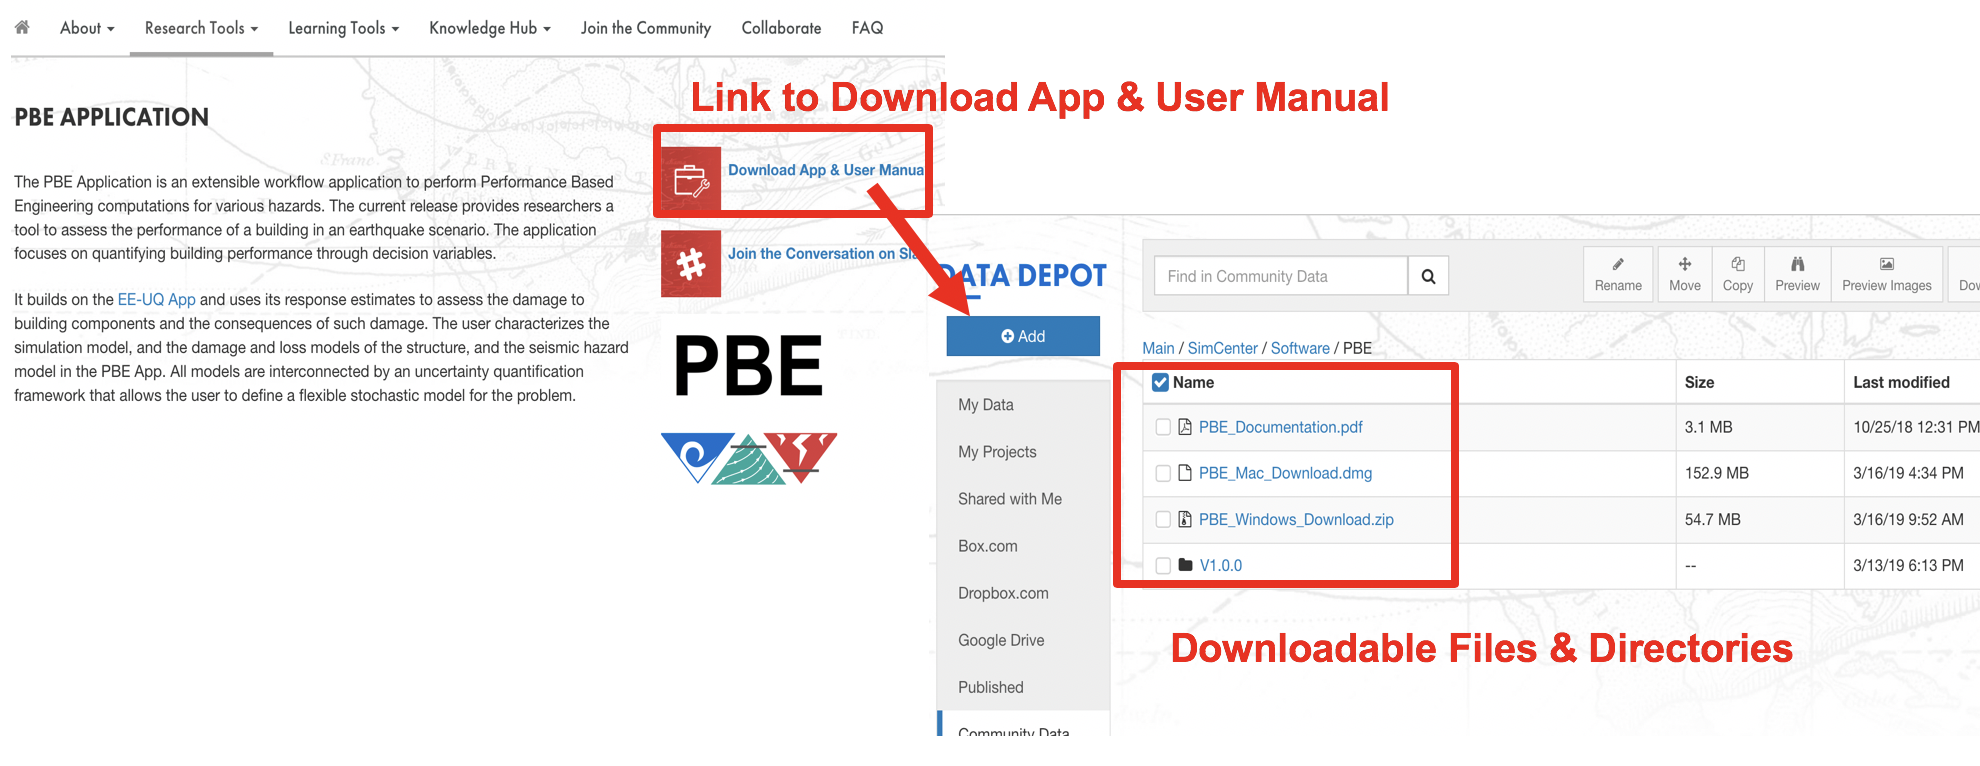
\includegraphics[width=0.95\textwidth]
    {installation/figures/pbeDownload.png} }
  \caption{Download Application.}
  \label{fig:app_choose_file}
\end{figure}
}{}

\softwareSwitch{EE-UQ}{
\begin{figure}[!htbp]
  \centering {
    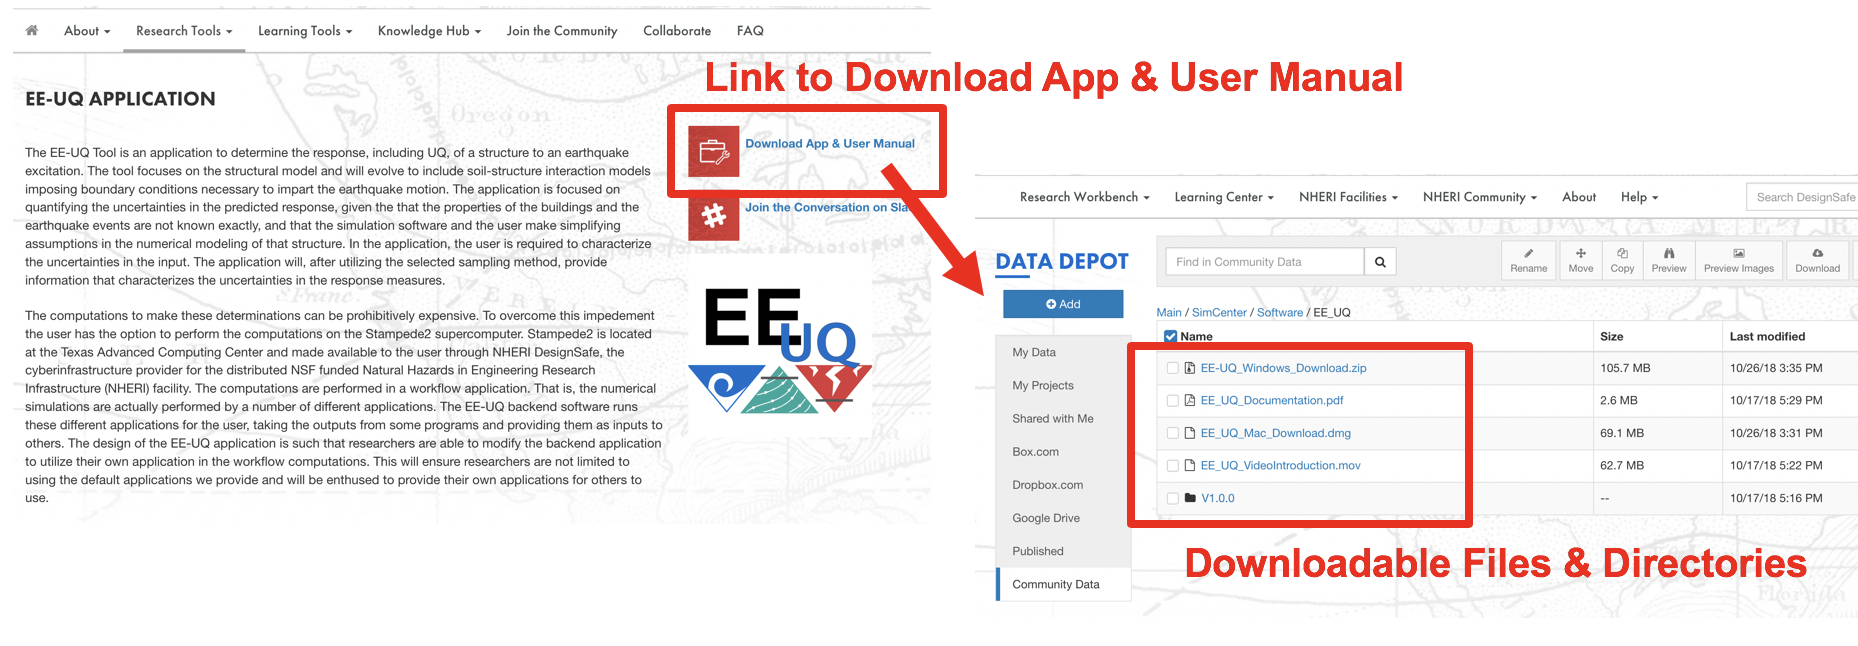
\includegraphics[width=0.95\textwidth]
    {installation/figures/eeDownload.png} }
  \caption{Download Application.}
  \label{fig:app_choose_file}
\end{figure}
}{}

\softwareSwitch{WE-UQ}{
\begin{figure}[!htbp]
  \centering {
    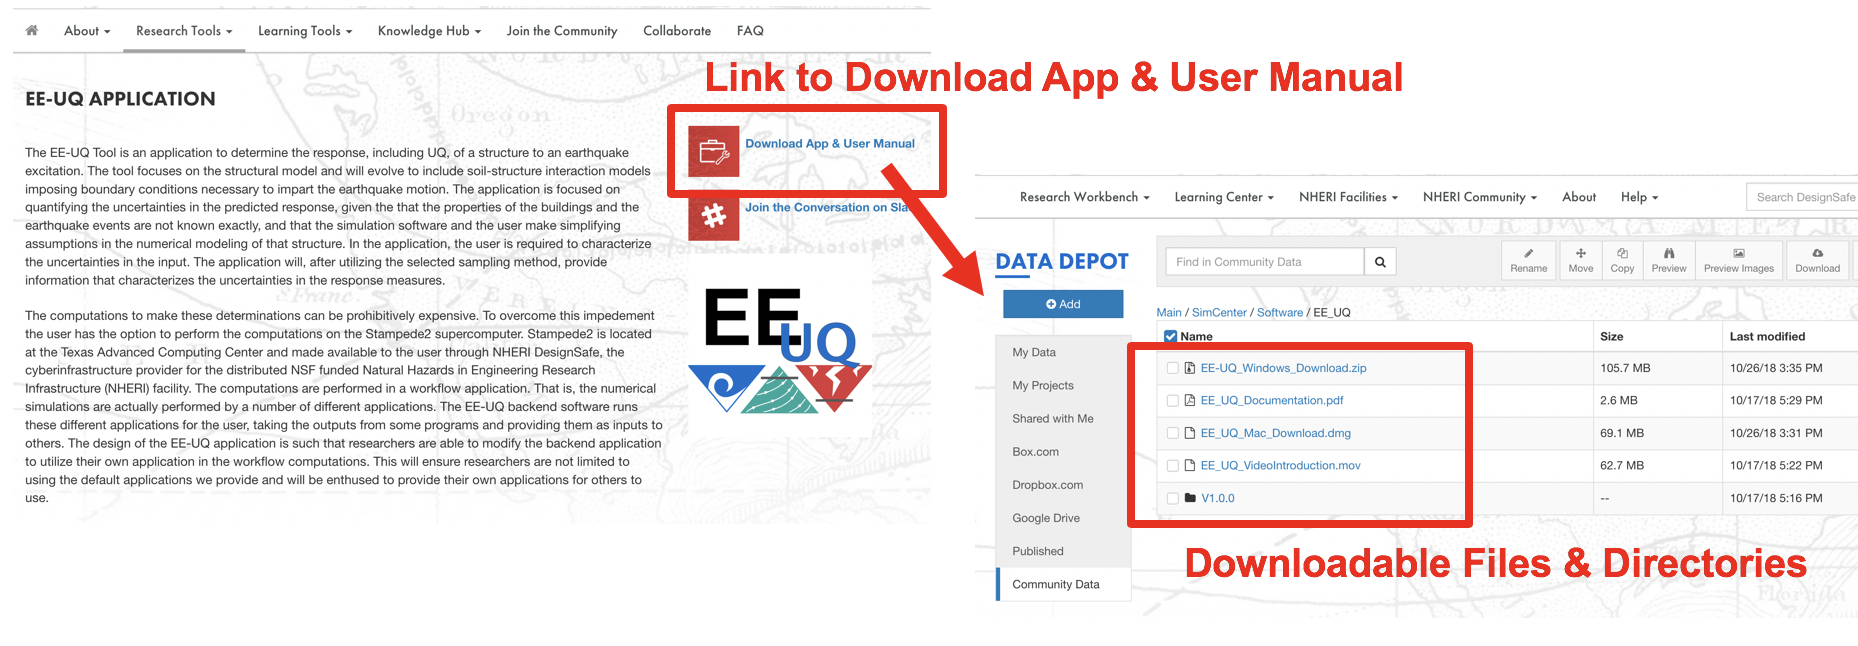
\includegraphics[width=0.95\textwidth]
    {installation/figures/eeDownload.png} }
  \caption{Download Application.}
  \label{fig:app_choose_file}
\end{figure}
}{}


There are at least four files available for download from this page: 
\begin{enumerate}
    \item The PDF file is the User Manual that you are reading now.
    \item The MOV file is an video that provides an introduction to the usage of the application.
    \item The ZIP file is an archive that contains the application files for a Windows operating system.
    \item The DMG file is an archive that contains the application files for a Mac OS X operating system.
\end{enumerate}

To download the \texttt{\getsoftwarename{}} application click on the link for
the appropriate file for your operating system and then click on the
Download button at bottom right corner of the ensuing pop-up window to
download it. You need to unpackage the application from the downloaded
file and place it in a location on your filesystem. On Windows, we
recommend that you create a \texttt{C:/SimCenter/\getsoftwarename{}}
directory and extract the contents of the \texttt{ZIP} archive
there. It is also recommended to run the included installer for Visual C/C++ runtime library(vc\_redist.x64.exe). On Mac, we recommend you copy the application to either your
Documents folder or your Desktop folder. You are free to place the
applications anywhere you wish, you will just need to make the
appropriate adjustments with the following instructions if you do so. \\

Now quickly test that the application starts. To do this navigate to
the location where you placed the application and open it. You should
see the user interface (UI) shown in \Cref{fig:app_UI} after
starting the application. Now Quit the application as there is more installtion steps required.\\

\softwareSwitch{PBE}{
\begin{figure}[!htbp]
  \centering {
    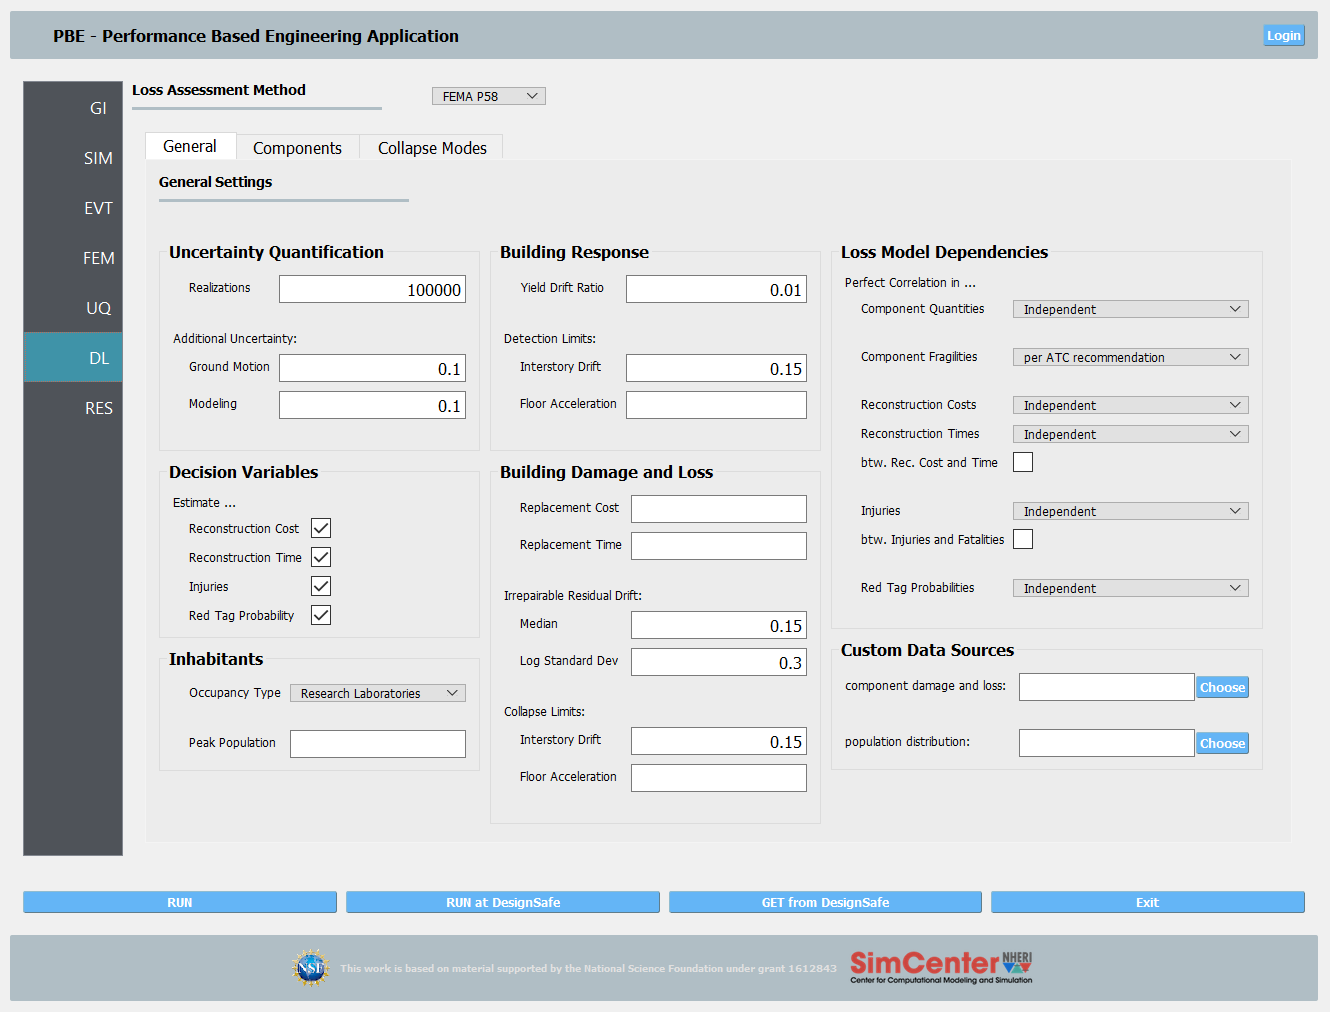
\includegraphics[width=0.95\textwidth]
    {installation/figures/PBE.png} }
  \caption{Running PBE Application.}
  \label{fig:app_UI}
\end{figure}
}{}

\softwareSwitch{EE-UQ}{
\begin{figure}[!htbp]
  \centering {
    \includegraphics[width=0.95\textwidth]
    {installation/figures/EE_UQ.png} }
  \caption{EE-UQ Application on Startup}
  \label{fig:app_UI}
\end{figure}
}{}

\softwareSwitch{WE-UQ}{
\begin{figure}[!htbp]
  \centering {
    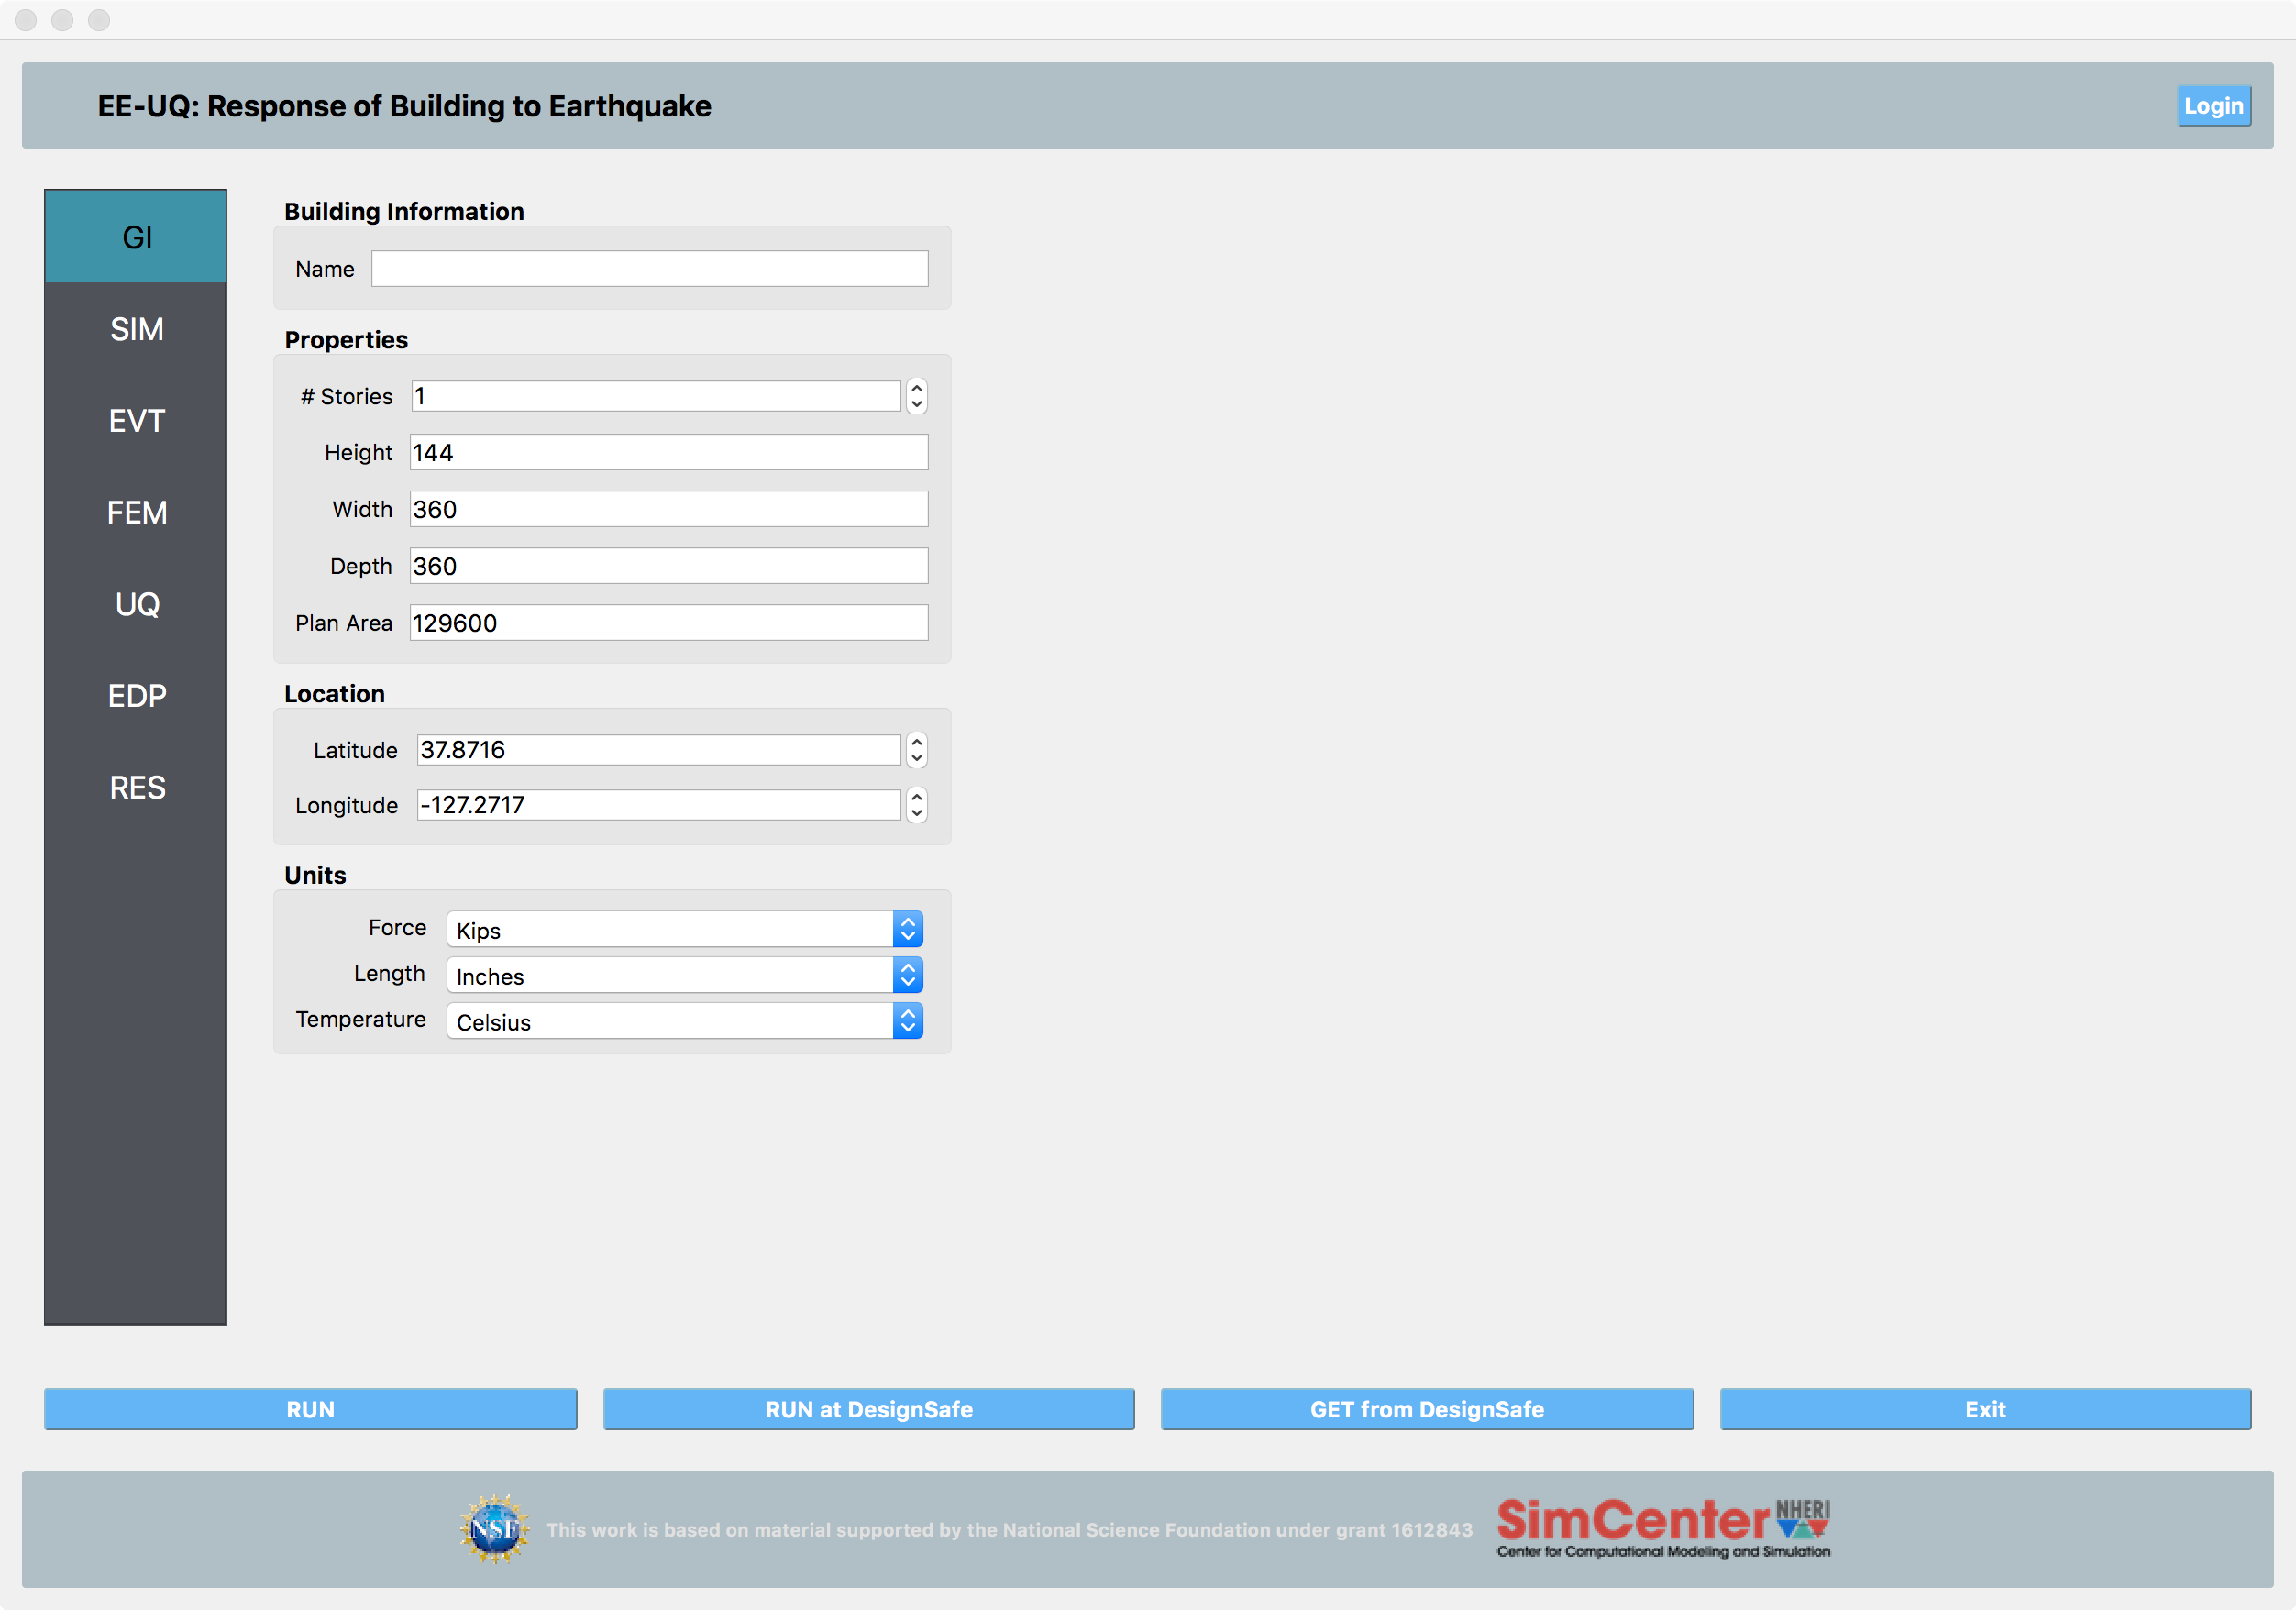
\includegraphics[width=0.95\textwidth]
    {installation/figures/EE-UQ.png} }
  \caption{EE-UQ Application on Startup}
  \label{fig:app_UI}
\end{figure}
}{}


\begin{enumerate}
\item The SimCenter is not recognized as either a Windows or an Apple vendor. Our applications are not recognized by the operating system as being signed. Consequently, you may receive a warning message when you start the \texttt{\getsoftwarename{}} application for the first time.
\item  On a Mac you will need to right click on the .dmg file to open it. Furthermore, the UI will not start correctly while in the DMG file, you need to open the .dmg file and then copy the \texttt{\getsoftwarename{}} application to your Documents or Desktop folder. You can then move the .dmg file to the trash or eject it after this has been done.
\item  The \texttt{\getsoftwarename{}} application requires additional software to work properly. Although the user interface loads, you will not be able to run calculations before installing those software.
\end{enumerate}



%===============================================================================
\section{Set up Python}
%===============================================================================

The SimCenter workflow applications are managed by Python
scripts. These are required to prepare the input data for running
analyses remotely on DesignSafe and also required for running
simulations locally. As a consequence the user must have Python
installed on their machine and have the appropriate environment
variables set so that the UI can run these applications.

\subsection{Install Python}

If you do not have a Python installation yet, we recommend
installing \href{http://www.anaconda.com/distribution/#download-section}{Anaconda}. Anaconda
provides all the important scientific packages in a single convenient
install. We recommend installing the 64-Bit version based on Python
3.5 or newer.

Note: If you already have a Python installation that is Python 2.7 or
newer, you do not have to install Anaconda to work with SimCenter
applications. You may also use another Python distribution. However,
if you do please make sure that you make the following packages
available: \texttt{numpy}, \texttt{scipy}, \texttt{pandas}.

\subsection{Test Python}
%===============================================================================

Test if the python environment is set up properly by
executing \texttt{python} in a terminal window. After Python starts,
test if the packages are installed by executing \texttt{import
numpy}, \texttt{import scipy}, and \texttt{import pandas}. You will
receive an error message if a pacakage is missing. If no error
appears, the terminal should look similar
to \Cref{fig:python_test}. Exit Python by executing
the \texttt{exit()} command.

\begin{figure}[!htbp]
  \centering {
    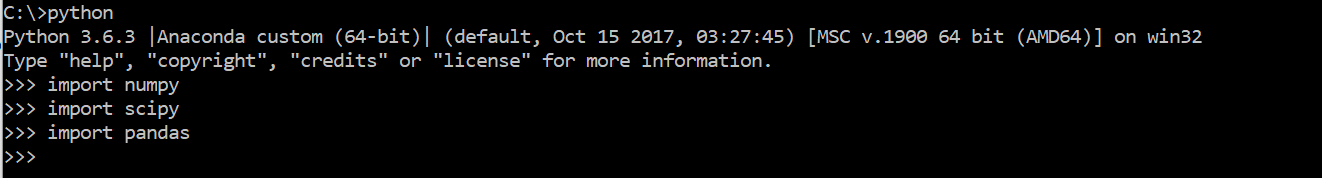
\includegraphics[width=0.8\textwidth]
    {installation/figures/python_test.png} }
  \caption{Testing the Python environment.}
  \label{fig:python_test}
\end{figure}

%===============================================================================
\section{Set up for Running Workflows Locally}\label{setup}
%===============================================================================

To run the workflows locally, the backend python application needs
publicly available software to also be installed on your
machine. These software applications need to be installed and
configured on your operating system. If you do not plan to run the
workflows locally, you will not need these applications.

\subsection{Install \texttt{OpenSees}}
%===============================================================================

\href{http://opensees.berkeley.edu}{\texttt{OpenSees}} is an open-source finite element application publicly available for download from its \href{http://opensees.berkeley.edu/OpenSees/user/download.php}{download page}. \texttt{OpenSees} installation requires the user install both \texttt{OpenSees} and \texttt{Tcl}.  If you have never downloaded \texttt{OpenSees} before, you will need to register your e-mail to gain access. After registration, you can proceed to the download page by entering your email address and clicking the Submit button. The Windows and Mac downloads are in different locations on the download page, with the appropriate Tcl installer beside the \texttt{OpenSees} link. This is as indicated in \Cref{fig:openseesDownload}

\begin{figure}[!htbp]
  \centering {
    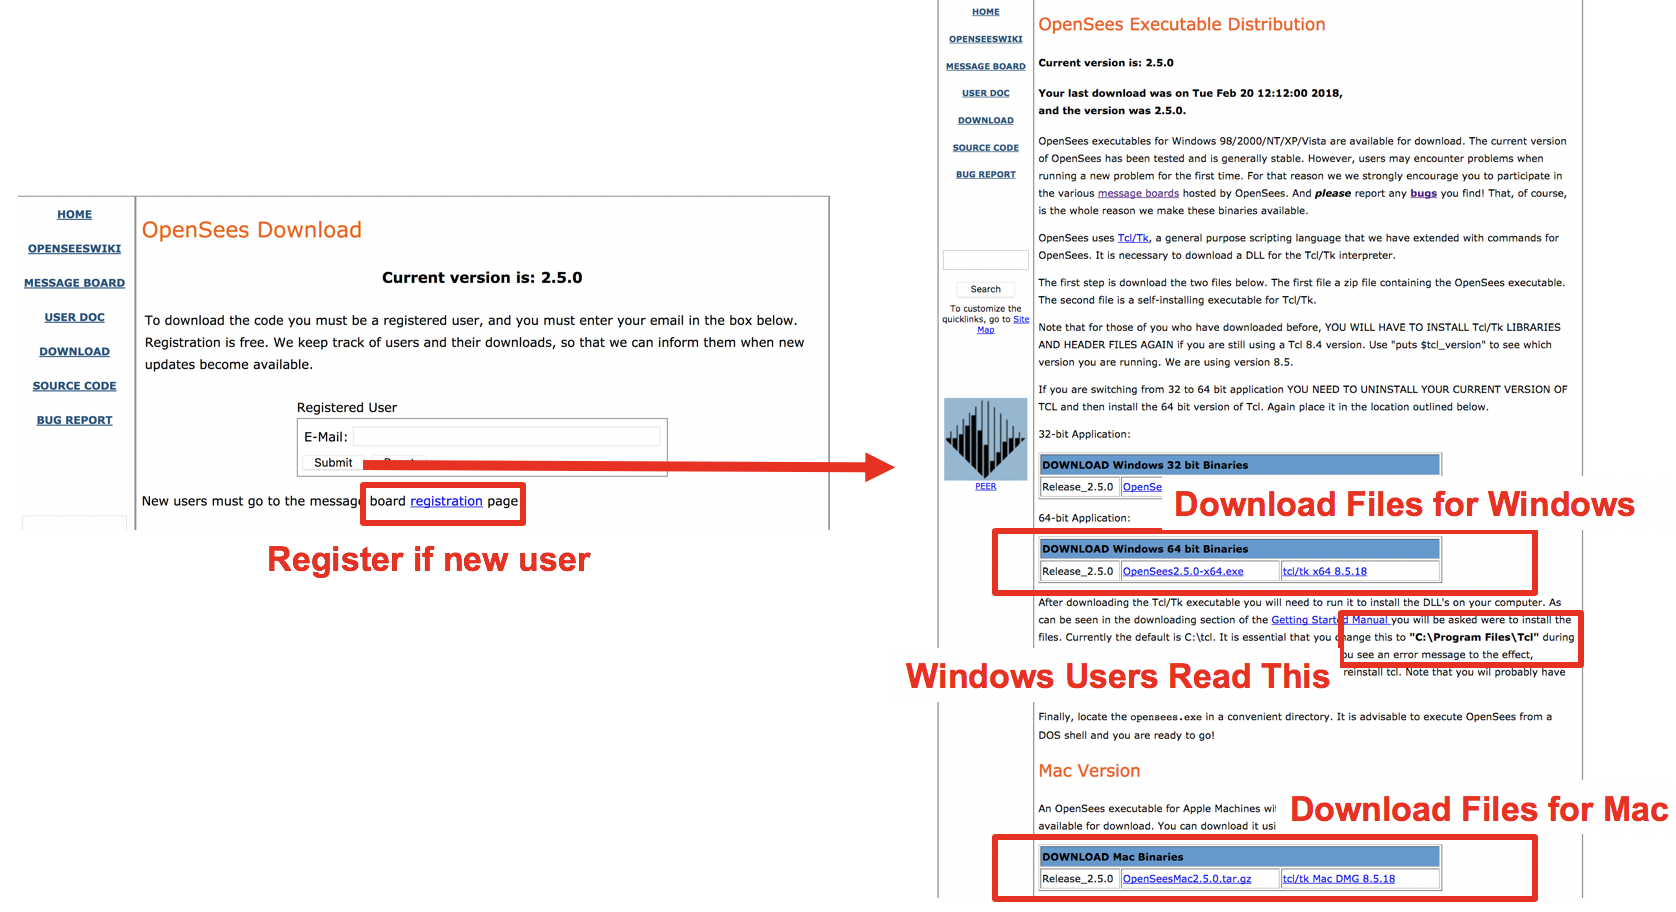
\includegraphics[width=\textwidth]
    {installation/figures/openseesDownload.png} }
  \caption{Downloading OpenSees}
  \label{fig:openseesDownload}
\end{figure}

Follow the instructions on the download page to install \texttt{Tcl}
(\Cref{fig:openseesDownload}). On Windows, pay particular
attention to the location \texttt{Tcl} must be installed in, as this is not the
default, and make sure you run the installer as administrator,
otherwise you will not be able to create the \texttt{C:/Program
Files/Tcl} folder.\\

After \texttt{Tcl} is installed, we recommend you put \texttt{OpenSees} in
the \texttt{C:/SimCenter/OpenSees} folder on Windows and in
a \texttt{/usr/local/OpenSees} directory on the Mac (If you use finder
on Mac to do navigation, use command-shift-G in Finder and specify
/usr/local as the folder to go to. There create a new folder \texttt{OpenSees}
and copy the \texttt{OpenSees} application to this folder).\\


Now you need to add the \texttt{OpenSees} folder to the
system \texttt{PATH} environment variable to allow the SimCenter
workflow applications to find the \texttt{OpenSees} executable on your
computer. The steps to do this depend on your operating system:

\begin{enumerate}
\item Windows: To add a folder to the \texttt{PATH} on Windows (\Cref{fig:add_env_path}):

\begin{figure}[!htbp]
  \centering {
    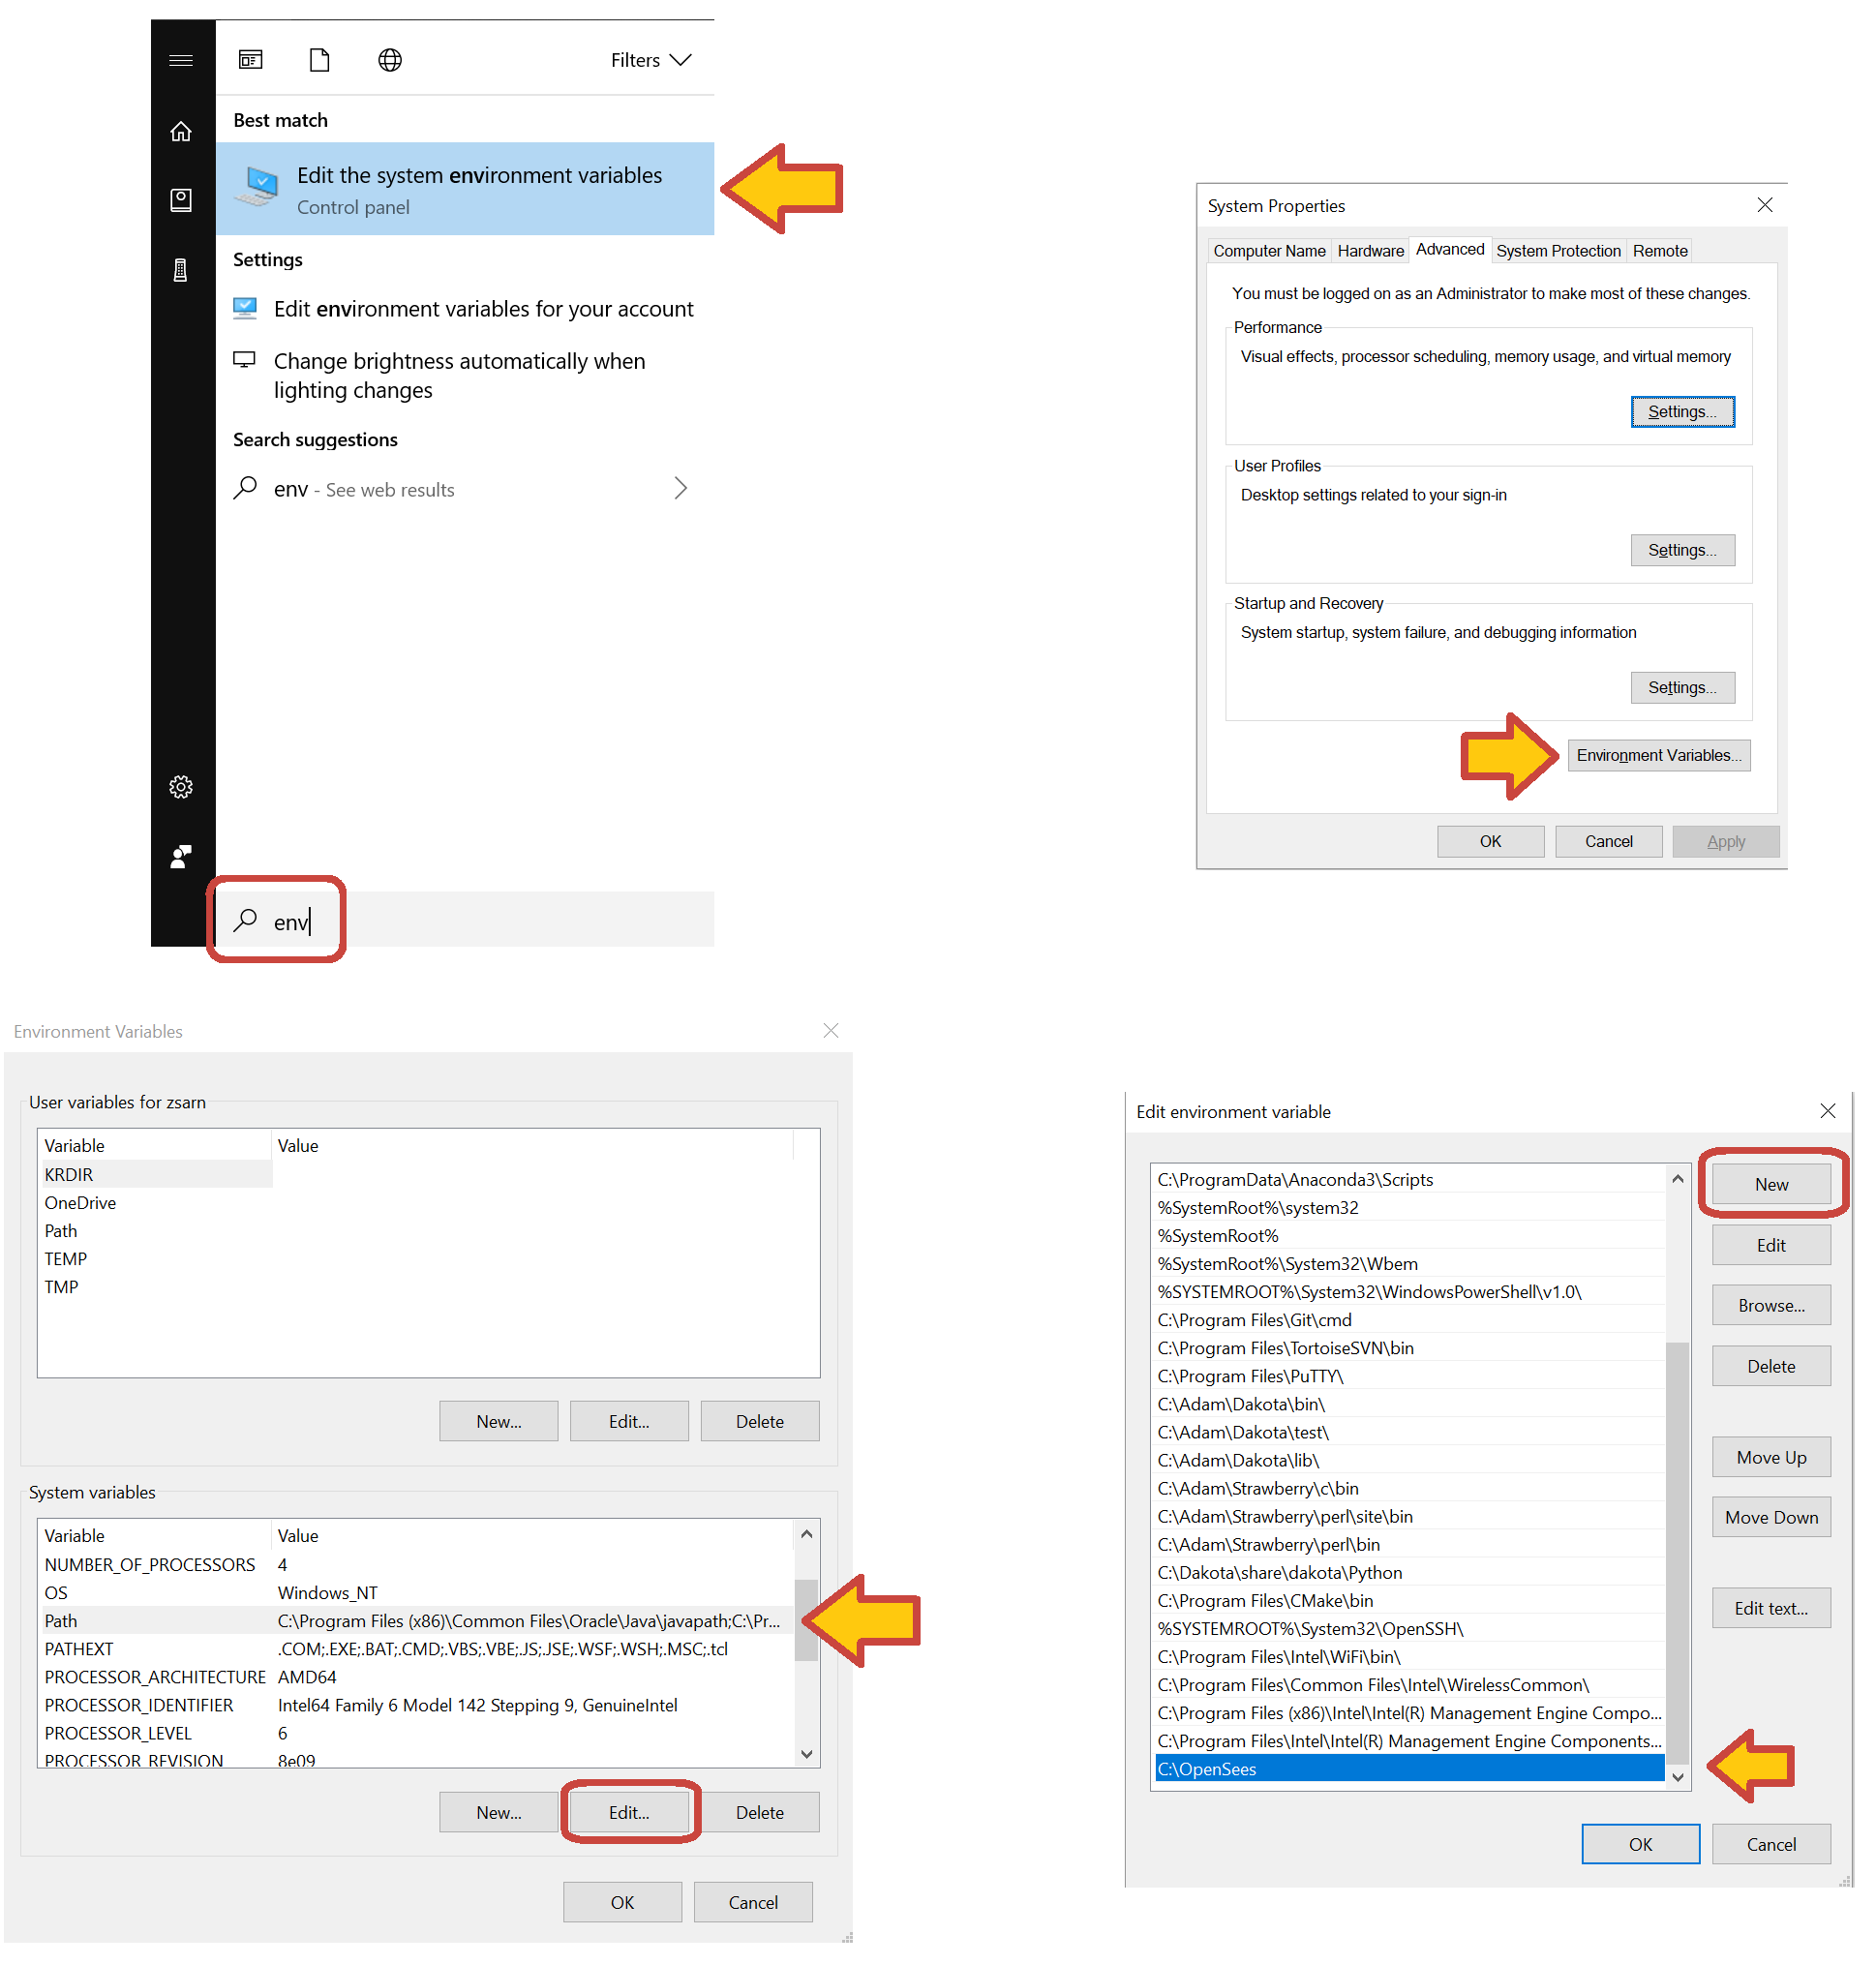
\includegraphics[width=0.8\textwidth]
    {installation/figures/add_env_path.png} }
  \caption{Adding OpenSees to the PATH environment variable on Windows.}
  \label{fig:add_env_path}
\end{figure}


\begin{enumerate}
    \item open \emph{Start}, type \emph{env}, and choose \emph{Edit the system environment variables};
    \item click on the \emph{Environment variables...} button in the dialog window;
    \item find the \texttt{Path} under \emph{System Variables} in the \emph{Variable} column;
    \item click \emph{New} and type in the path to your \texttt{OpenSees.exe} (this will be \texttt{C:\textbackslash SimCenter\textbackslash OpenSees} if you put the executable at the recommended location - pay attention to using backslashes here!);
    \item click \emph{OK} in every dialog to close them and save your changes.
\end{enumerate}

\item MacOS: To add the /usr/local/OpenSees folder to the \texttt{PATH} variable::


\begin{enumerate}
    \item open a Terminal;
    \item execute \texttt{sudo nano /etc/paths} and enter your password
    \item add the path to the \texttt{OpenSees} executable to the end of the list (this will be \texttt{/usr/local/OpenSees} if you put the executable at the recommended location);
    \item quit by hitting \texttt{Ctrl+X} and then \texttt{Y} when asked if you want to save modifications.
\end{enumerate}

\begin{figure}[!htbp]
  \centering {
     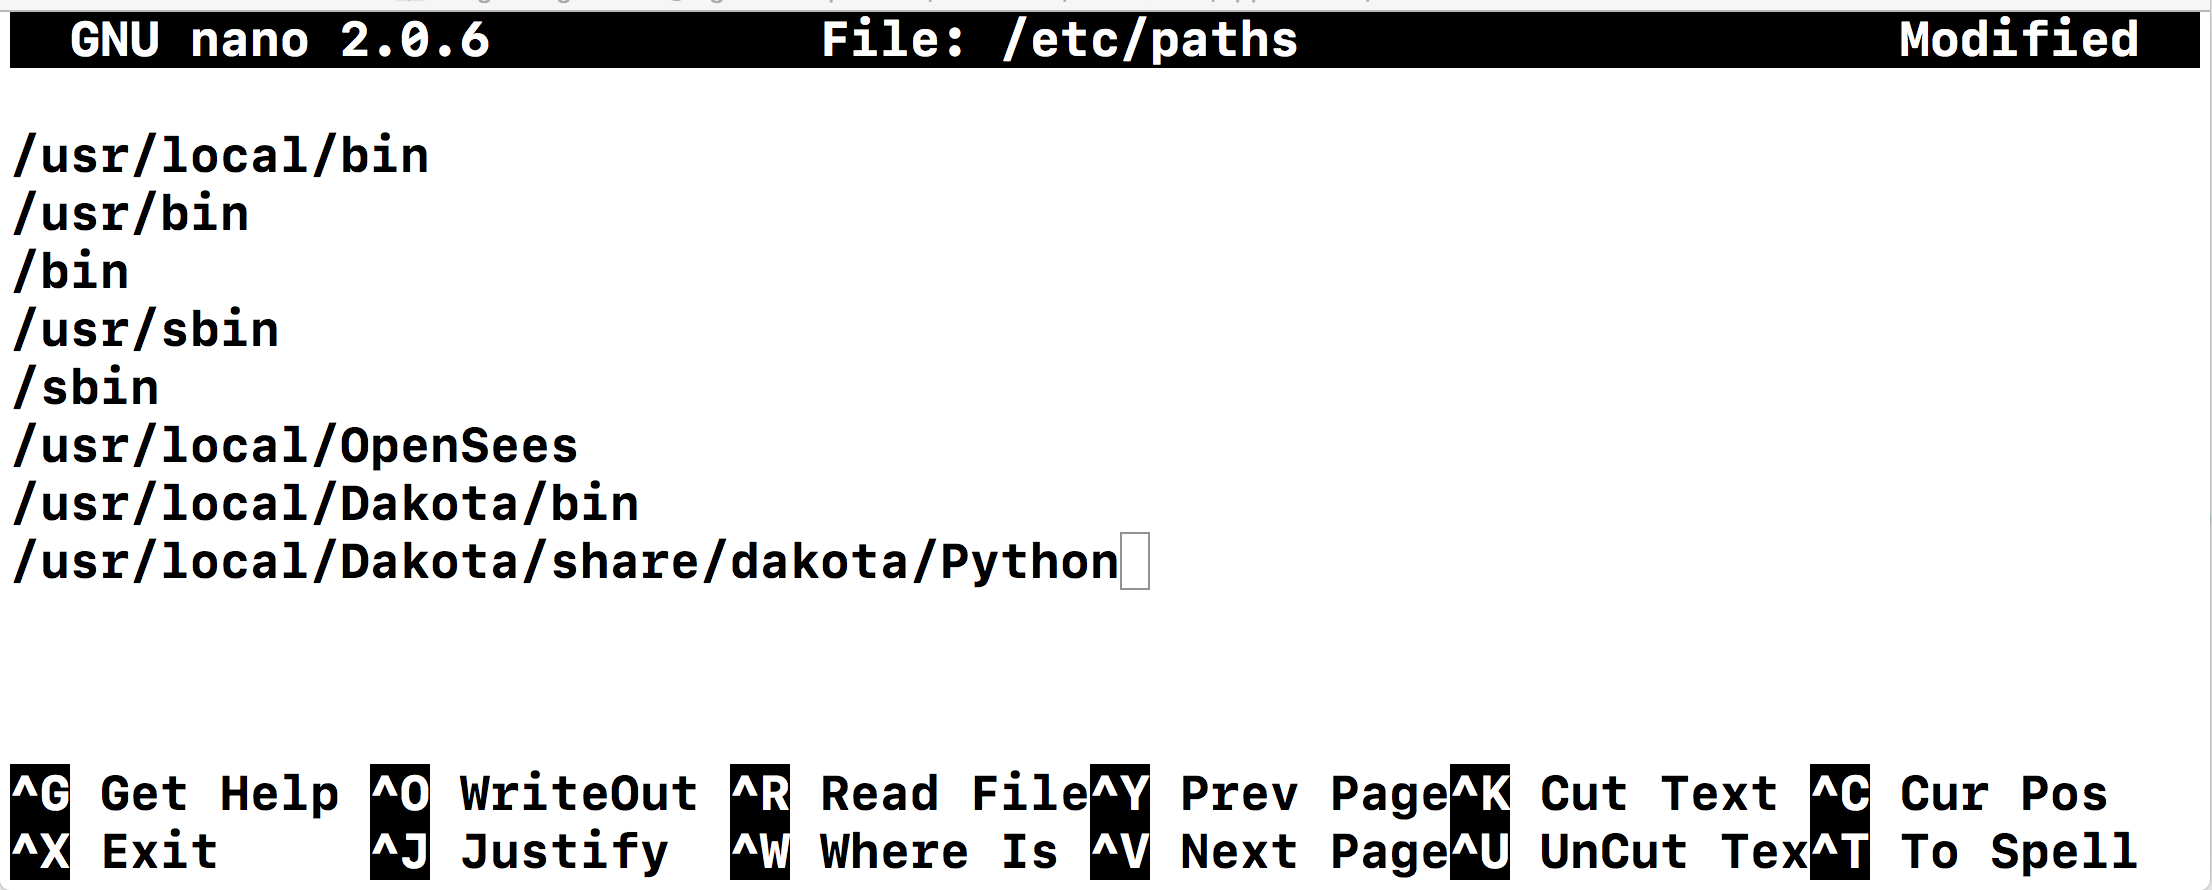
\includegraphics[width=0.8\textwidth]
    {installation/figures/add_env_path_Mac.png} }
  \caption{Adding OpenSees to the PATH environment variable on Mac.}
  \label{fig:add_env_path_Mac}
\end{figure}
\end{enumerate}


\subsection{Install \texttt{Dakota}}
%===============================================================================

\href{http://dakota.sandia.gov}{\texttt{Dakota}}, an open-source  optimization and UQ application from Sandia National Labs, is publicly available for download at its \href{http://dakota.sandia.gov/download.html}{download page}. Select your operating system from the list and set the other options as shown in  \Cref{fig:dakota_installation}. Download the release in a \texttt{ZIP} file for Windows and \texttt{TAR.GZ} file for Mac. We recommend you to extract the archive to a \texttt{C:/SimCenter/Dakota} folder on Windows, and to a \texttt{/usr/local/Dakota} folder on a Mac.

\begin{figure}[!htbp]
  \centering {
    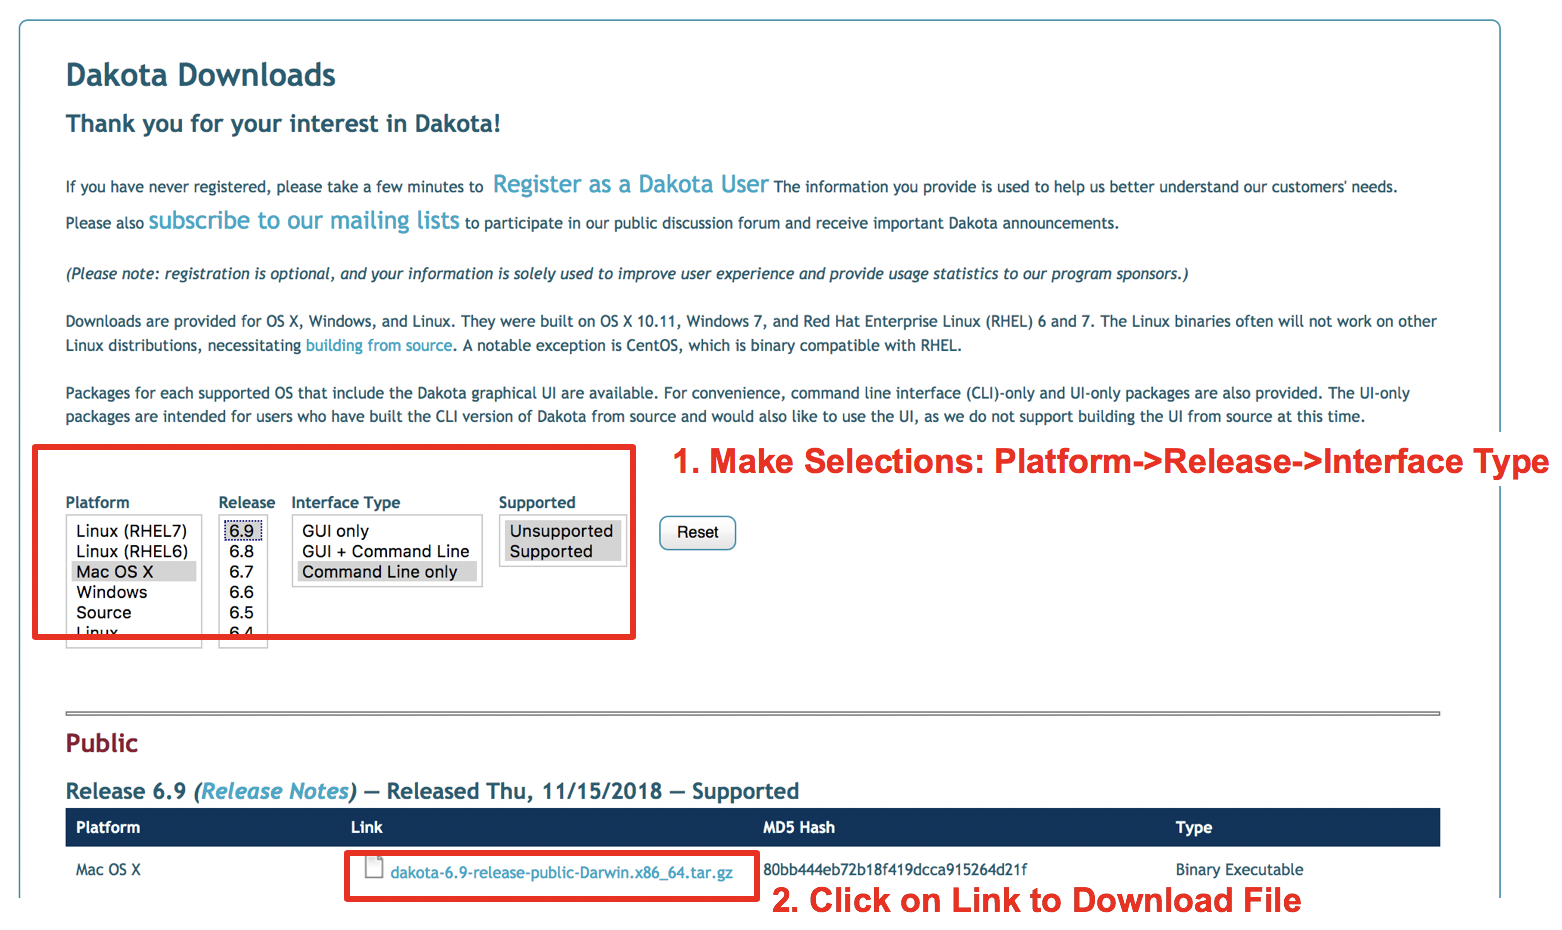
\includegraphics[width=\textwidth]
    {installation/figures/dakota_installation.png} }
  \caption{Downloading Dakota Software}
  \label{fig:dakota_installation}
\end{figure}

Following the instructions provided for installing \texttt{OpenSees}, you need to add \textbf{two} \texttt{Dakota} folders to the
system \texttt{PATH} environment variable to allow the SimCenter
workflow applications to find the \texttt{Dakota} tools on your computer. Use
the procedure described above for \texttt{OpenSees} to add the following
folders to your \texttt{PATH}:

\begin{enumerate}
\item Windows:
\begin{itemize}
    \item \texttt{C:\textbackslash SimCenter\textbackslash Dakota\textbackslash bin}
    \item \texttt{C:\textbackslash SimCenter\textbackslash Dakota\textbackslash share\textbackslash dakota\textbackslash Python}
\end{itemize}

\item MacOS:
\begin{itemize}
    \item \texttt{/usr/local/Dakota/bin}
    \item \texttt{/usr/local/Dakota/share/dakota/Python}
\end{itemize}
\end{enumerate}
\subsection{Install  Perl}
%===============================================================================

Mac OS X has Perl pre-installed, but Windows users will have to
install it to be able to use \texttt{Dakota}. We recommend you use Strawberry
Perl; you can install it by downloading the executable from
its \href{http://strawberryperl.com}{Strawberry Perl website} and
running it.

\subsection{Test the Install of the Local Applications}
%===============================================================================

Before running the \texttt{\getsoftwarename{}} application, perform the following tests to
make sure that the local SimCenter working environment is set up
appropriately:

\begin{itemize}
    \item Start a Terminal on Mac or a Command Prompt on Windows.
    \item On Mac, execute \texttt{cd /usr/Documents} to change the active directory to \texttt{/usr/Documents}. On Windows, execute \texttt{cd C:/} to change the active directory to \texttt{C:/}.
    \item Test if \texttt{OpenSees} works correctly by executing the \texttt{OpenSees} command. The command should start \texttt{OpenSees} (\Cref{fig:opensees_test}). Close \texttt{OpenSees} with the \texttt{exit} command.
    \item Test if \texttt{Dakota} works correctly by executing the \texttt{dakota} command. The command should start \texttt{Dakota} and you should see a message about a missing argument (\Cref{fig:dakota_test}).
    \item Test if Perl works correctly by executing the \texttt{perl -v} command. The command should start Perl and return its version number (\Cref{fig:perl_test}).
    \item Test if the python package in \texttt{Dakota} works correctly by starting Python with the \texttt{python} command and then executing the \texttt{import dakota} command. This should import the dakota package. If you do not see errors, then the package is successfully imported (\Cref{fig:dakota_py_test}). Exit Python with the \texttt{exit()} command.
    \item If all the above tests ran without errors, your environment is set up appropriately.
\end{itemize}

\begin{figure}[!htbp]
  \centering {
    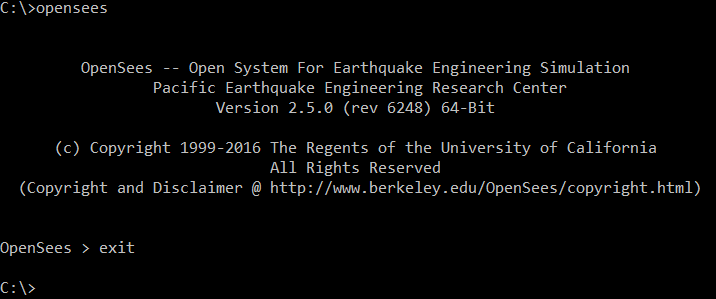
\includegraphics[width=0.8\textwidth]
    {installation/figures/opensees_test.png} }
  \caption{Testing OpenSees.}
  \label{fig:opensees_test}
\end{figure}

\begin{figure}[!htbp]
  \centering {
    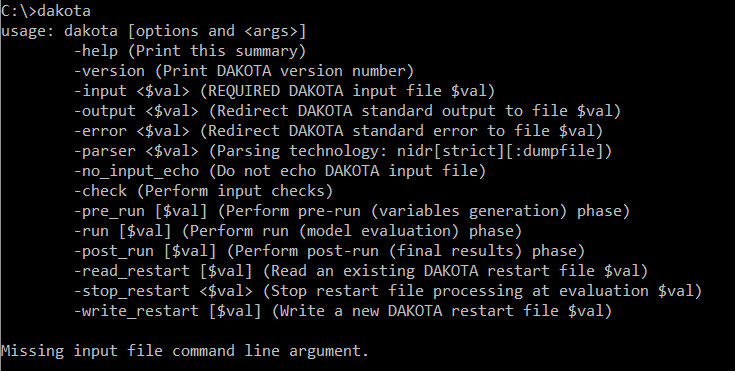
\includegraphics[width=0.8\textwidth]
    {installation/figures/dakota_test.png} }
  \caption{Testing Dakota.}
  \label{fig:dakota_test}
\end{figure}

\begin{figure}[!htbp]
  \centering {
    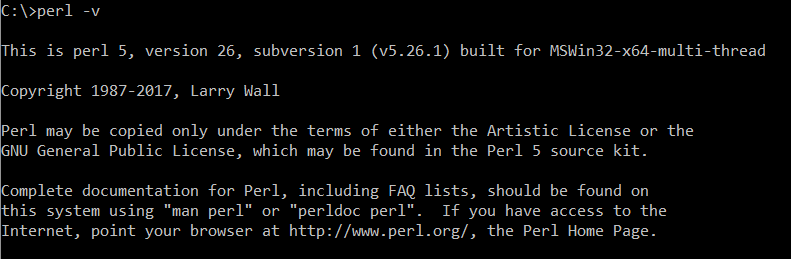
\includegraphics[width=0.8\textwidth]
    {installation/figures/perl_test.png} }
  \caption{Testing Perl.}
  \label{fig:perl_test}
\end{figure}

\begin{figure}[!htbp]
  \centering {
    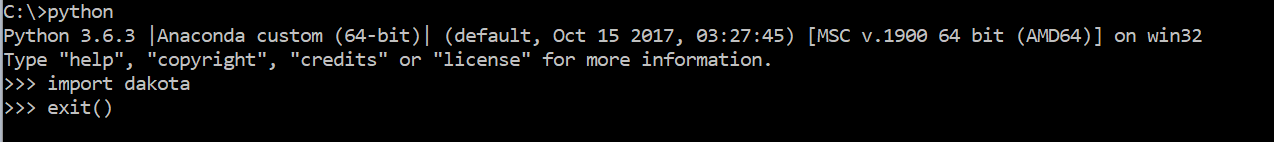
\includegraphics[width=0.8\textwidth]
    {installation/figures/dakota_py_test.png} }
  \caption{Testing the dakota Python package.}
  \label{fig:dakota_py_test}
\end{figure}

%===============================================================================
\clearpage
\section{Test the \texttt{\getsoftwarename{}} application}
\label{sec:test_local}
Once the local SimCenter working environment has been tested and is
functioning correctly, the \texttt{\getsoftwarename{}} Application
can be tested. The simplest way to do this is by running an analysis
using the default structural model with synthetic ground motions. By
doing this, it is not necessary to enter any information on the
structural model and only inputs for 
\softwareSwitch{PBE}{
the synthetic motions, uncertainty quantification, and loss assessment
}{
the synthetic motions and uncertainty quantification
}
are required. With this quick setup, the
functionality of the \texttt{\getsoftwarename{}} App and the backend
workflow can be tested. The necessary steps to perform this
testing are provided below.

A full description of how to use this software is provided
in \Cref{chap:usage}.  In this quick test, users will only
interface with the event tab (\texttt{EVT}), the uncertainty
quantification tab (\texttt{UQ}), 
\softwareSwitch{PBE}{
the damage and loss assessment tab (\texttt{CMP}),
}{}
and the results tab (\texttt{RES}).

The first step is to start the \texttt{\getsoftwarename{}}
application.  Once the application started, the second step is to
input the parameters for the synthetic motions under the \texttt{EVT}
(Event) tab. This is shown in \Cref{fig:input_event}. Click
on the \texttt{EVT} tab which will allow the loading type to be
selected. From the dropdown menu, as shown
in \Cref{fig:input_event}, select \texttt{Stochastic Ground Motion
Model}. Upon selecting this loading type, the loading model will be
set as \texttt{Vlachos et al. (2018)}.

\softwareSwitch{PBE}{
\begin{figure}[!htbp]
  \centering {
    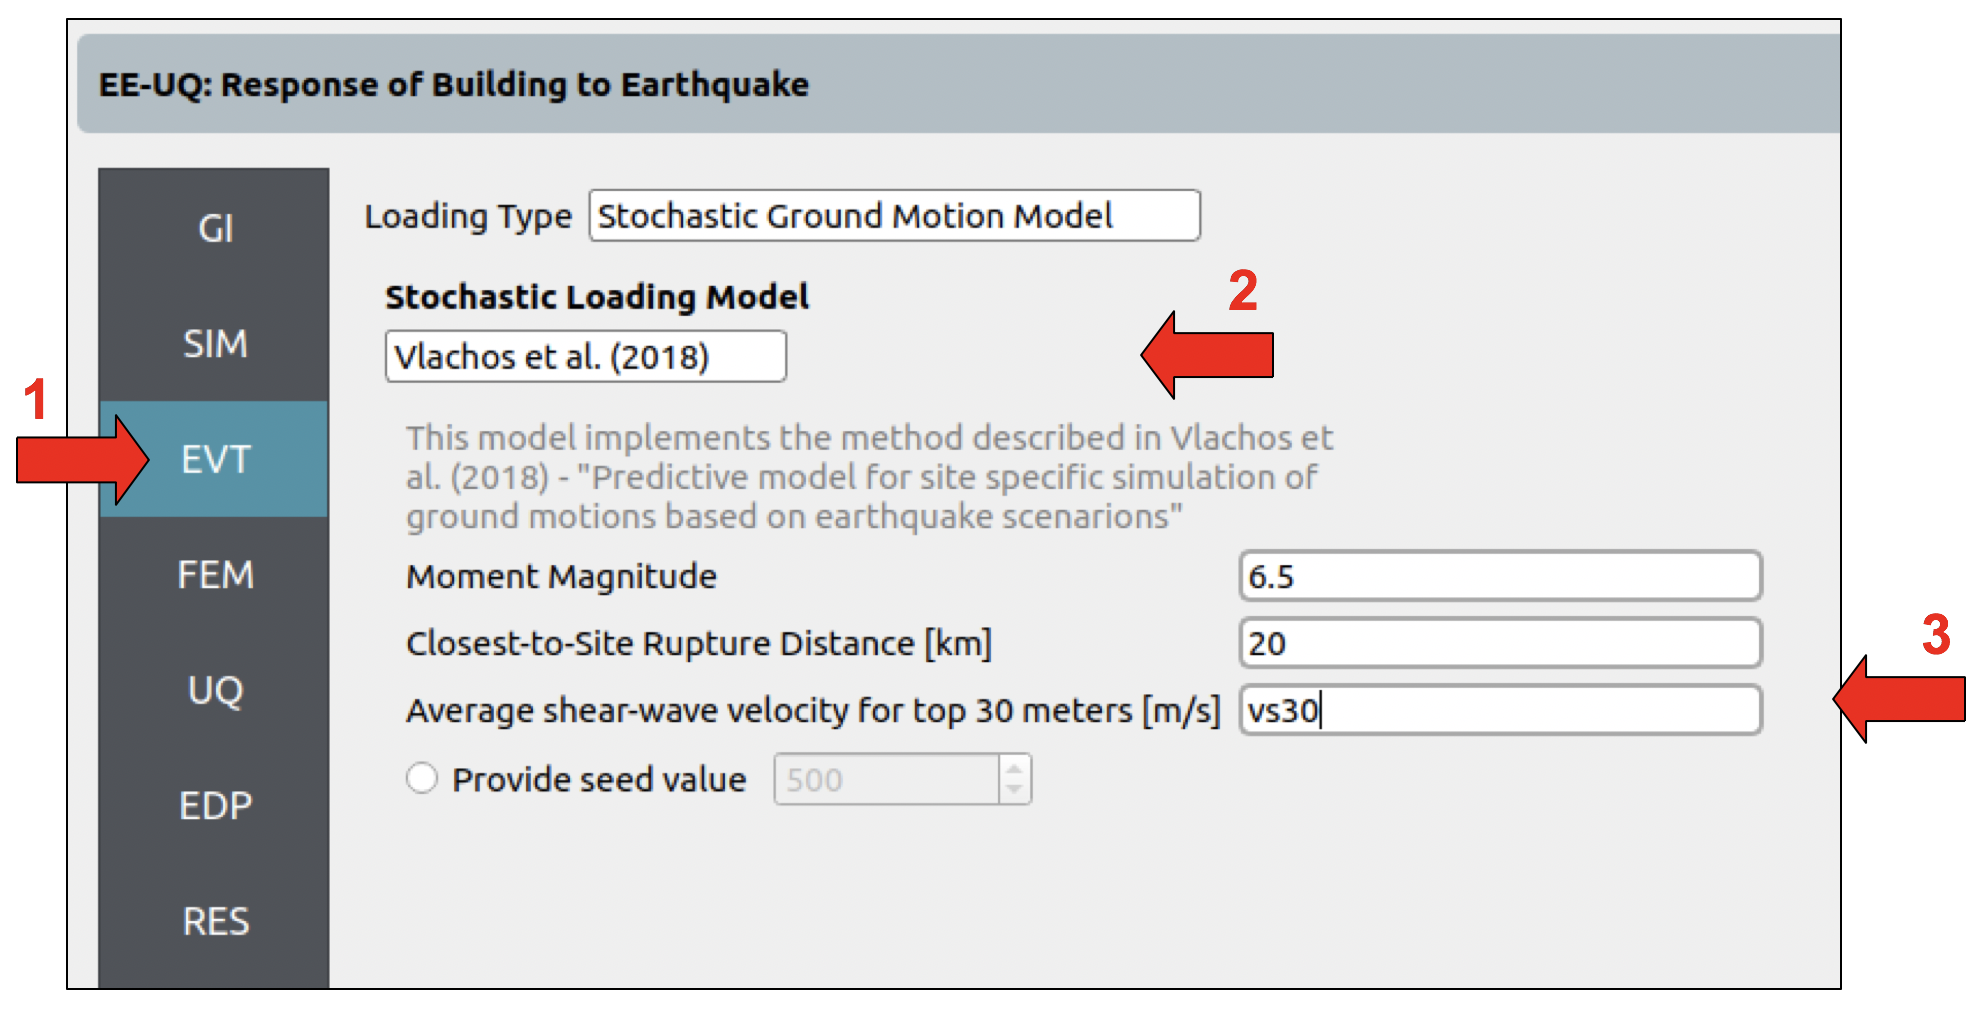
\includegraphics[width=0.7\textwidth]
    {installation/figures/test_input_event.png} }
  \caption{Selecting event type and inputting synthetic motion parameters}
  \label{fig:input_event}
\end{figure}
}{
\begin{figure}[!htbp]
  \centering {
    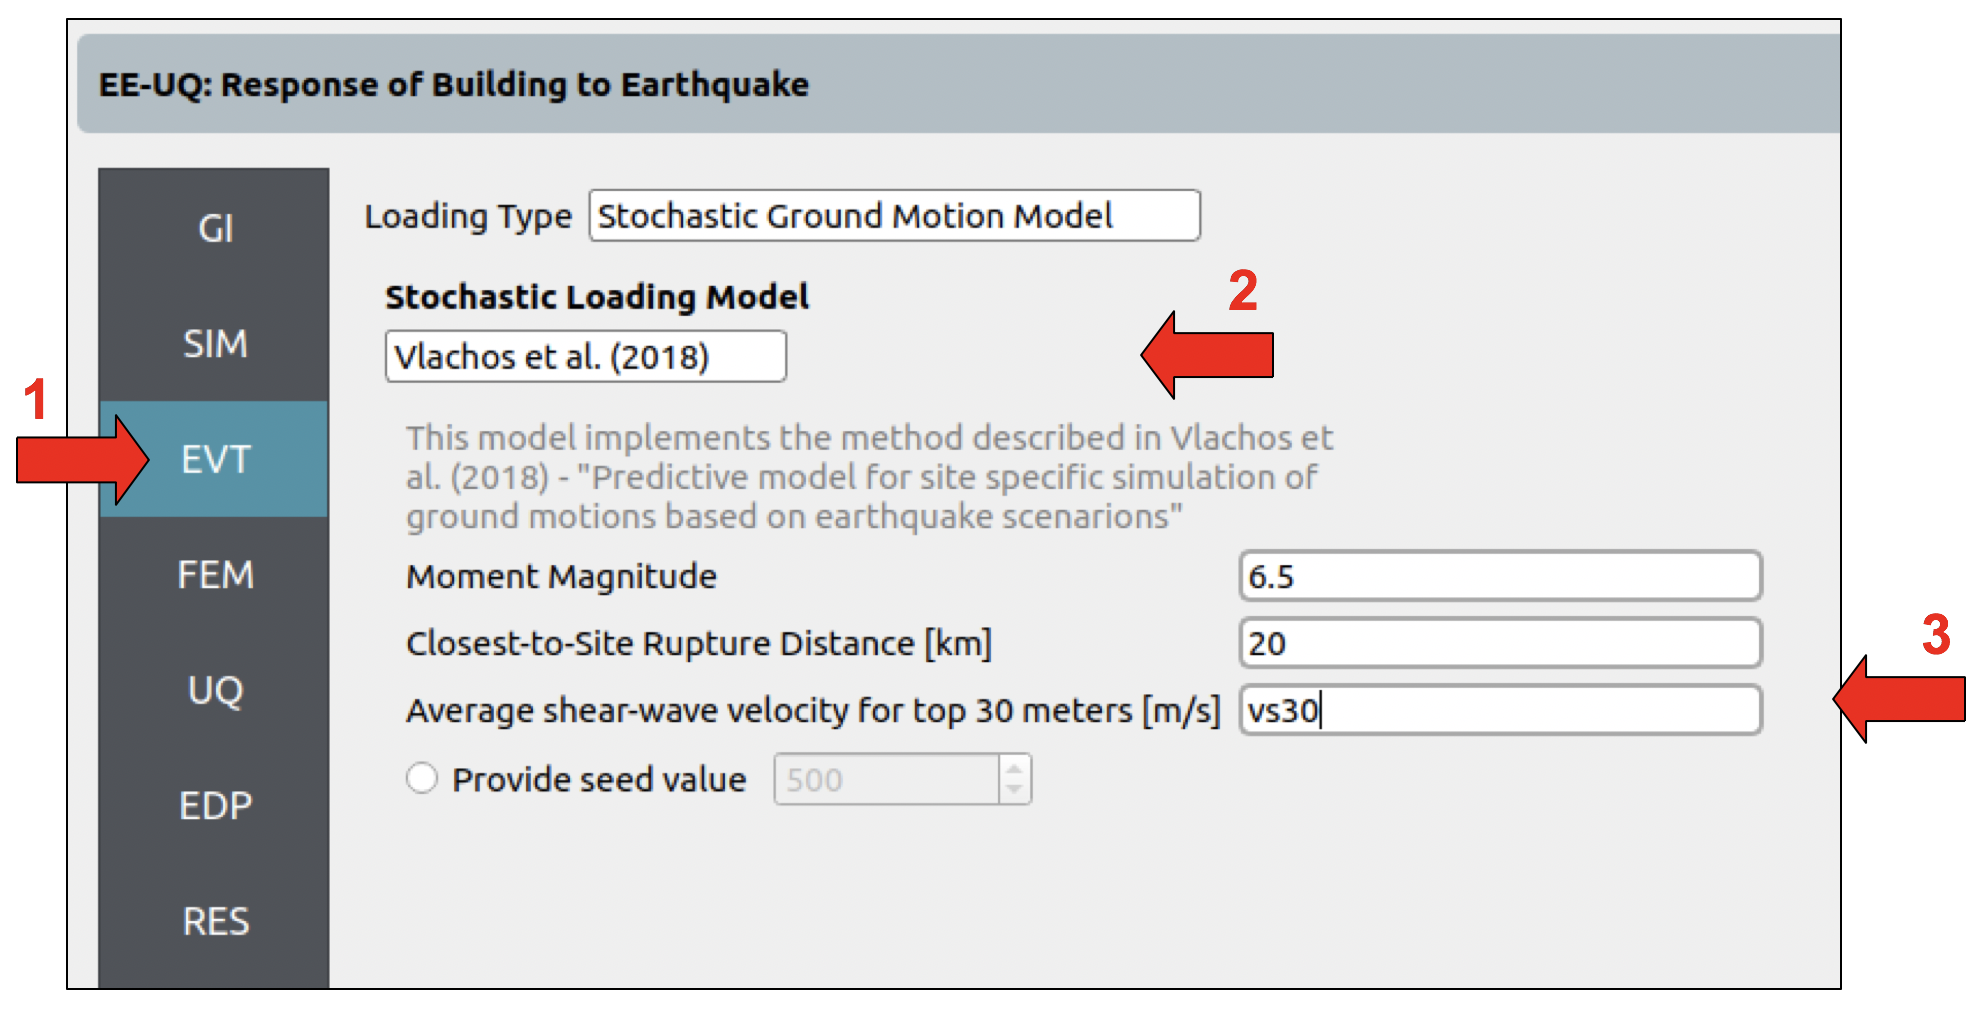
\includegraphics[width=0.7\textwidth]
    {installation/figures/test_input_event.png} }
  \caption{Selecting event type and inputting synthetic motion parameters}
  \label{fig:input_event}
\end{figure}
}

Only three inputs are required for this test, of which one will be set
to a random variable. As shown in \Cref{fig:input_event}, set the
\emph{Moment Magnitude} ($M_W$) to 6.5, the \emph{Closest-to-Site Rupture Distance}
($R_{rupt}$) to 20 km, and the \emph{Average shear-wave velocity
for the top 30 m} ($V_{S_{30}}$)
to \texttt{vs30}. The \texttt{Provide seed value} radio button should
be left unselected. By specifying these inputs, both $M_{W}$ and $R_{rupt}$
will have constant values in all realizations while $V_{S_{30}}$ will
have different values based on the model parameters specified in the
uncertainty quantification (\texttt{UQ}) tab.

With these inputs specified, navigate to the \texttt{UQ} tab. Here the
distributions and their relevant parameters will be specified for the
random variables defined in the analysis\textemdash only $V_{S_{30}}$
in this case. Since $V_{S_{30}}$ was identified as a random variable
by inputting the parameter value as text, it is automatically added as
a random variable, as shown in \Cref{fig:input_uq}. Set the
distribution type to \texttt{normal} with a \texttt{Mean}
and \texttt{Standard Dev} of 350 m/s and 25 m/s,
respectively.

\softwareSwitch{PBE}{
\begin{figure}[!htbp]
  \centering {
    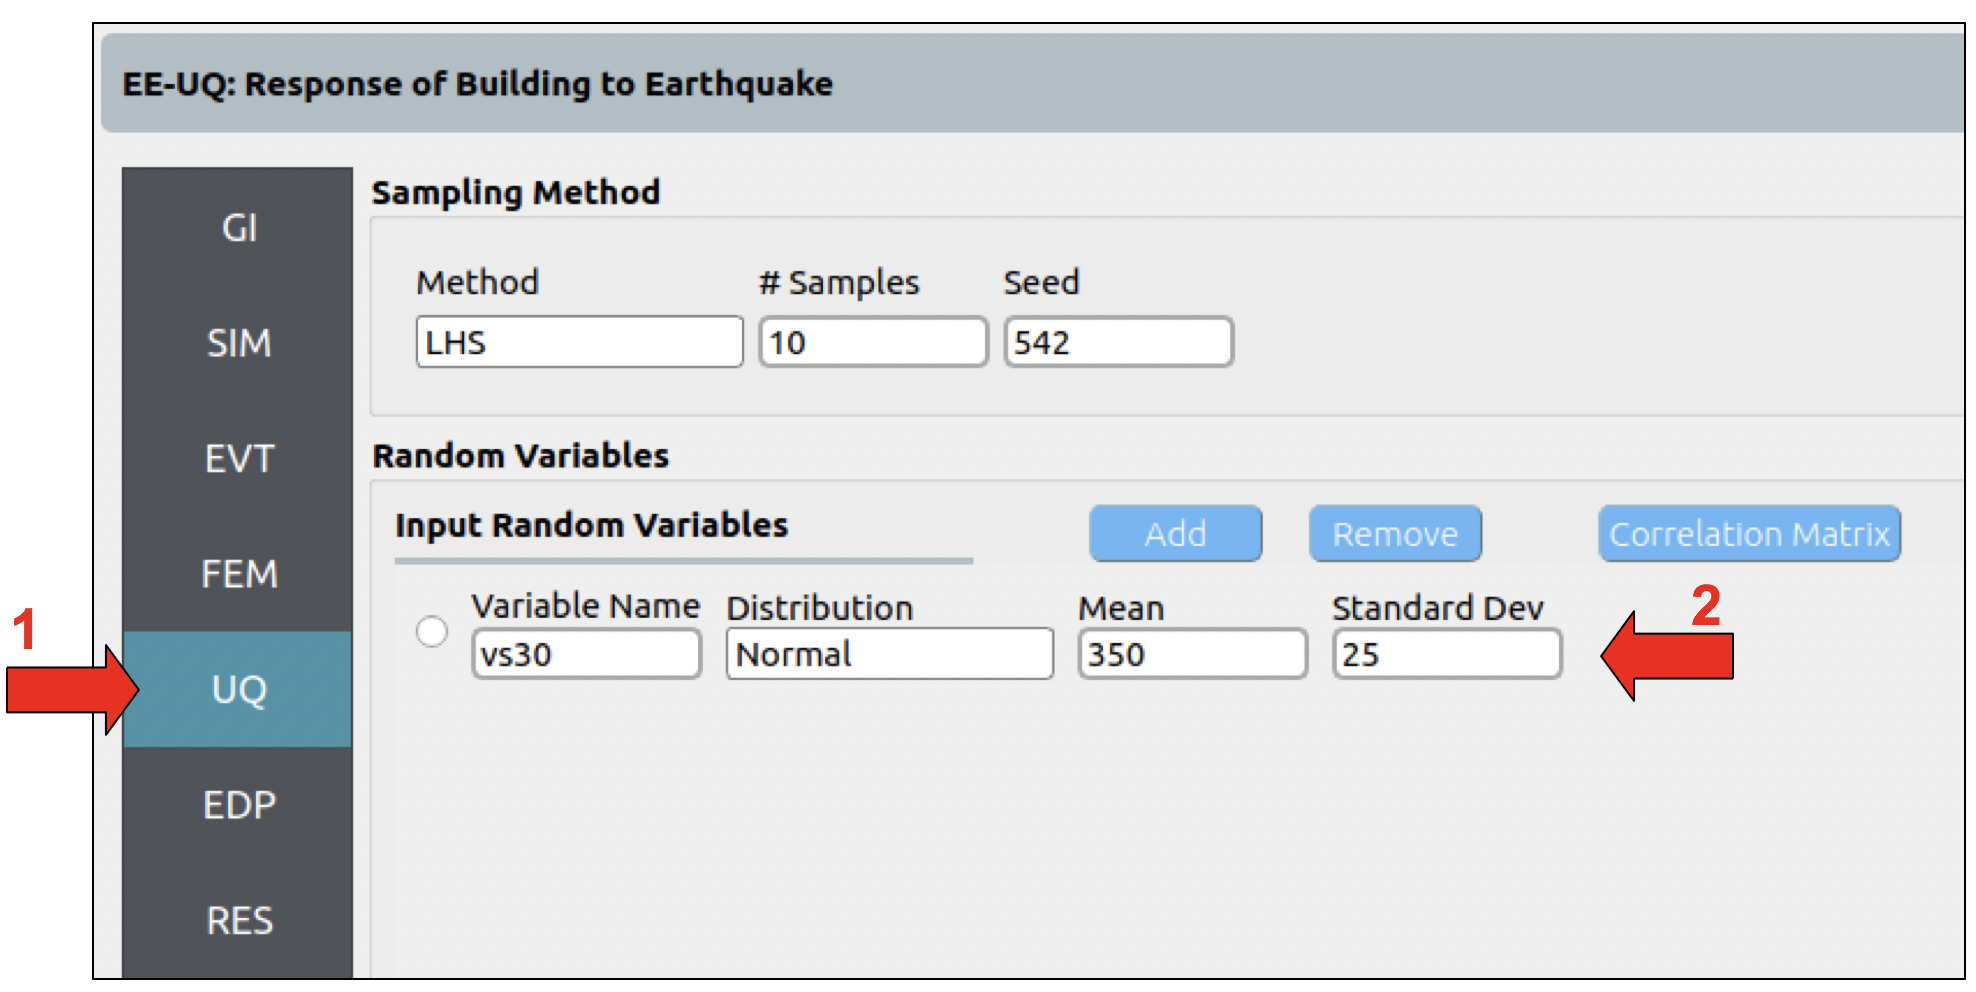
\includegraphics[width=0.7\textwidth]
    {installation/figures/test_input_uq.png} }
  \caption{Specifying distribution type and parameters for random
  variables in analysis\textemdash only $V_{s30}$ in this case}
  \label{fig:input_uq}
\end{figure}
}{
\begin{figure}[!htbp]
  \centering {
    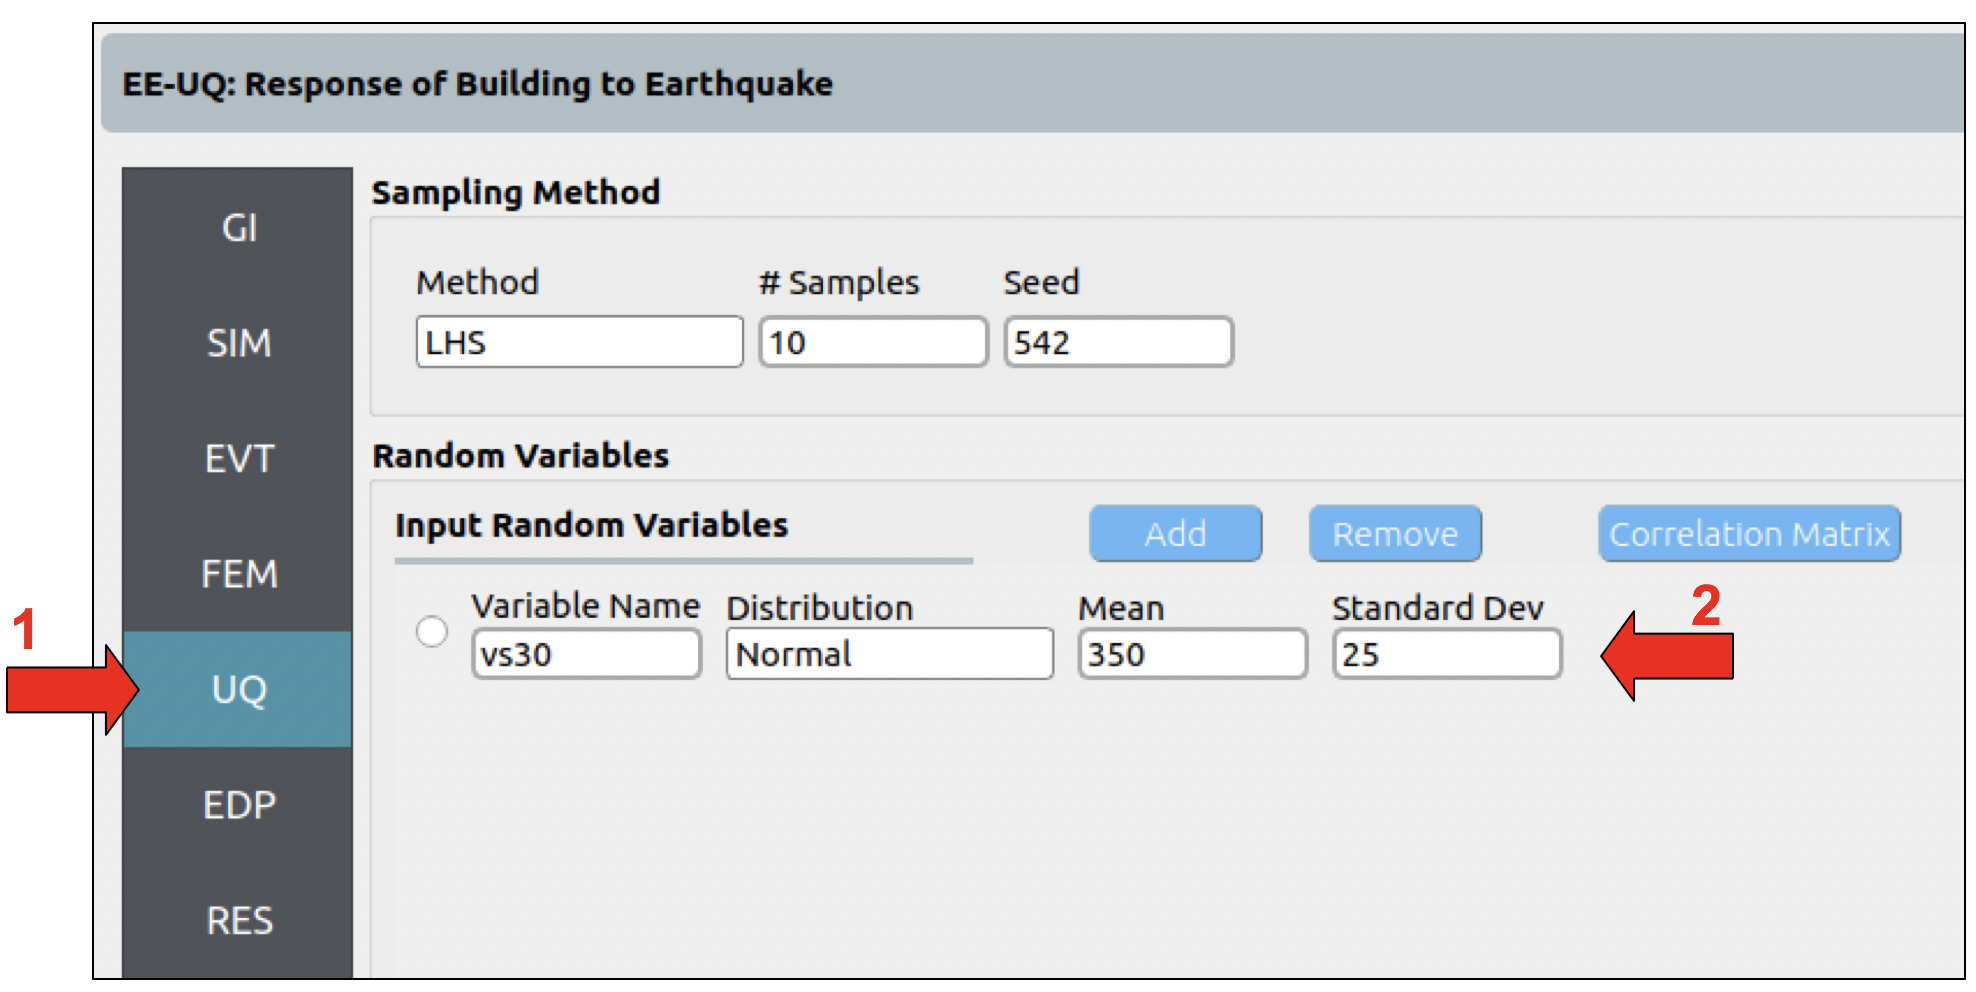
\includegraphics[width=0.7\textwidth]
    {installation/figures/test_input_uq.png} }
  \caption{Specifying distribution type and parameters for random
  variables in analysis\textemdash only $V_{s30}$ in this case}
  \label{fig:input_uq}
\end{figure}
}

\softwareSwitch{PBE}{
The last step before running the analysis is to set up a damage and loss model. Navigate to the \textttt{CMP} tab and select \texttt{HAZUS MH} as the loss assessment method to use. Set up the model according to \Cref{fig:input_dl}.
\begin{figure}[!htbp]
  \centering {
    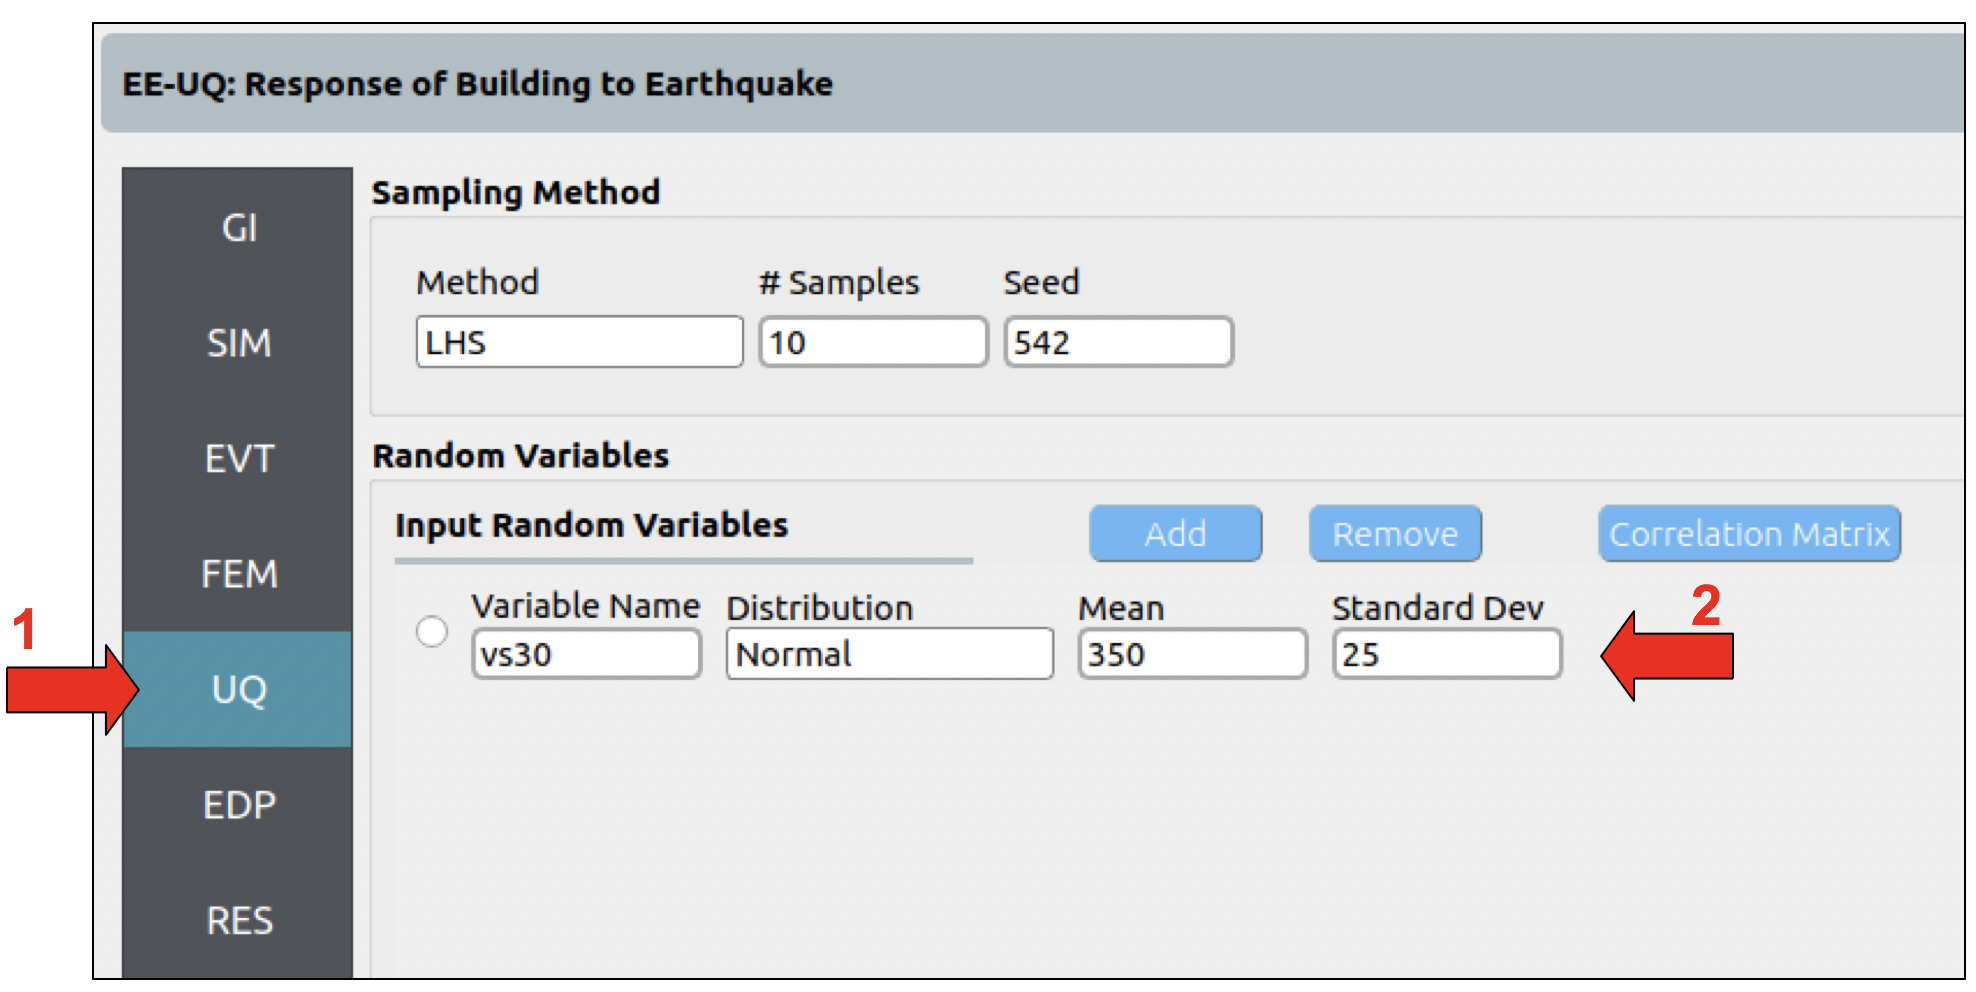
\includegraphics[width=0.7\textwidth]
    {installation/figures/test_input_uq.png} }
  \caption{Specifying the damage and loss model for the analysis.}
  \label{fig:input_dl}
\end{figure}
}{}

Now, click on the \texttt{RUN} button, which will bring up a pop-up
menu that provides information on the application directory and
the working directory. The application directory should already be
automatically set to where \texttt{\getsoftwarename{}} is installed.
If desired, the working directory can be changed. In order to start
the analysis, click on the \texttt{Submit} button.

\softwareSwitch{PBE}{
\begin{figure}[!htbp]
  \centering {
    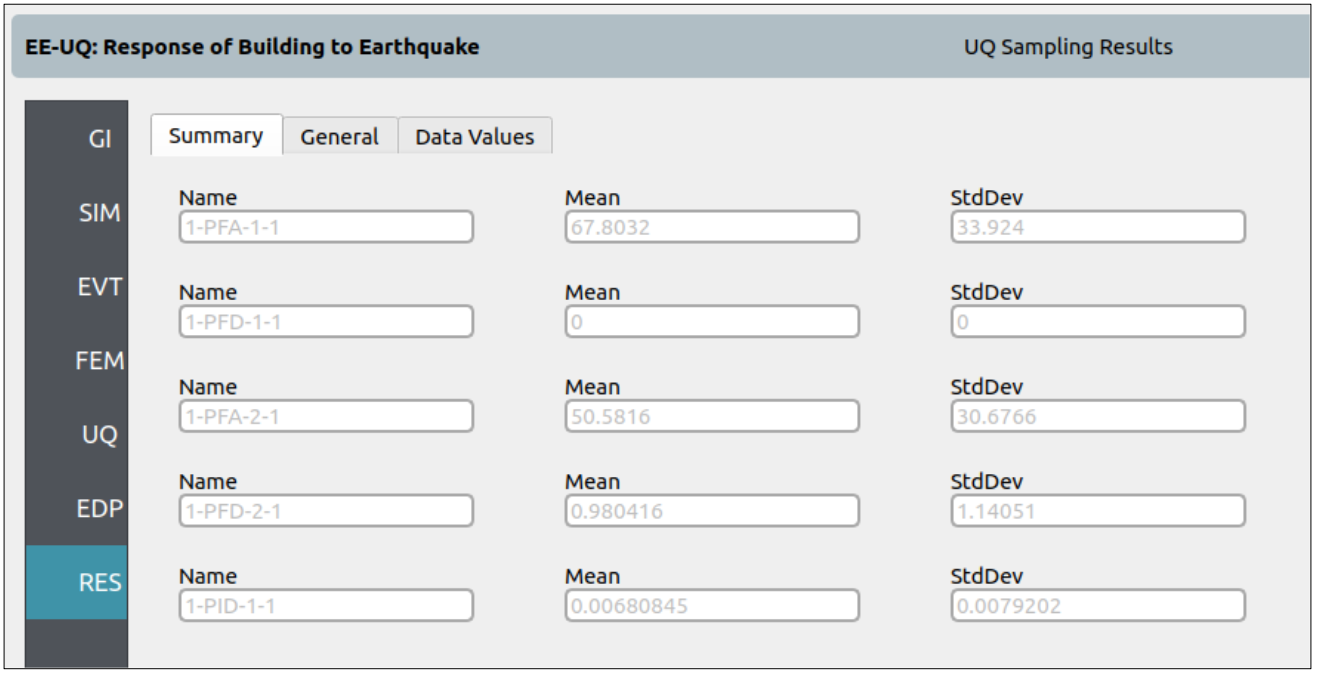
\includegraphics[width=0.7\textwidth]
    {installation/figures/test_uq_res.png} }
  \caption{Results for test analysis. This tab will open automatically
  when the analysis completes, indicating a successful installation}
  \label{fig:show_results}
\end{figure}
}{
\begin{figure}[!htbp]
  \centering {
    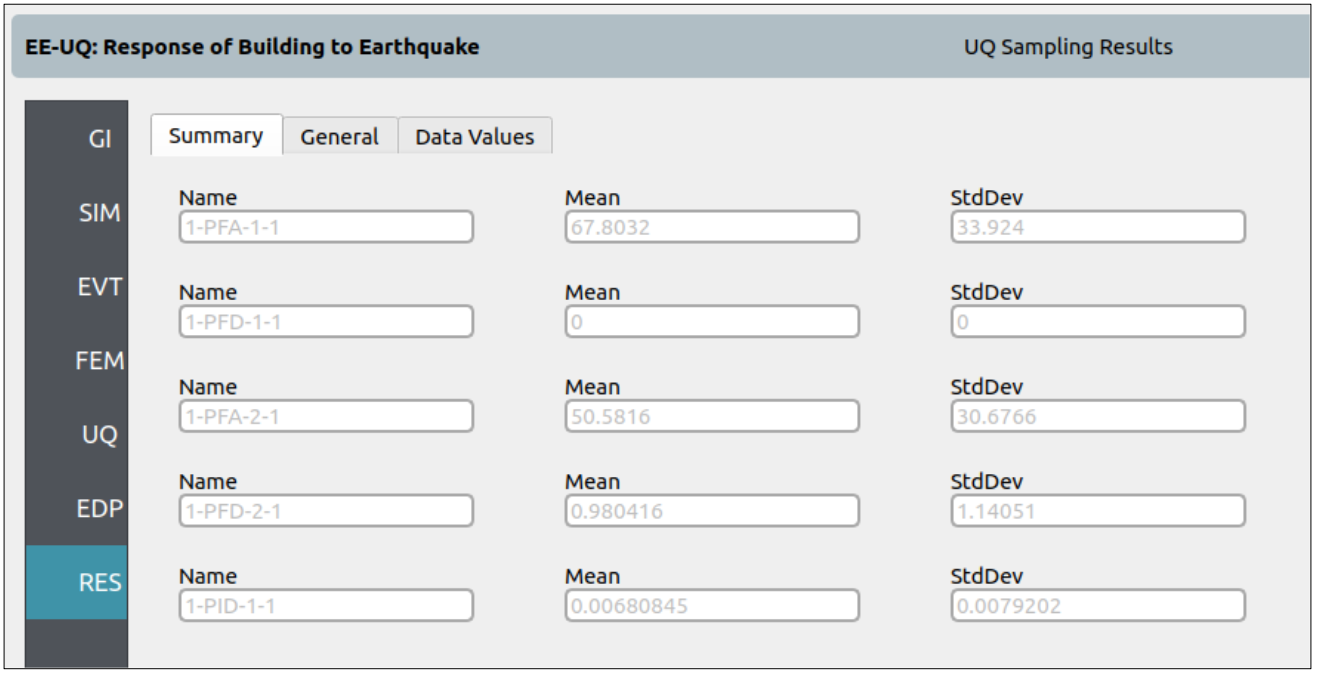
\includegraphics[width=0.7\textwidth]
    {installation/figures/test_uq_res.png} }
  \caption{Results for test analysis. This tab will open automatically
  when the analysis completes, indicating a successful installation}
  \label{fig:show_results}
\end{figure}
}

If successful, the application will pause briefly while it runs the
analysis before automatically displaying the simulations results in
the \texttt{RES} tab, as shown
in \Cref{fig:show_results}. Remember, the results shown
in \Cref{fig:show_results} most likely will not be the same as
those from this local test since $V_{S_{30}}$ is a random variable and
the values realized in the simulations will be different while still
following the same distribution. In any case, if the simulations
completed and the \texttt{RES} tab is showing simulation results, then
the \texttt{\getsoftwarename{}} App is properly installed and configured.

%===============================================================================
